\documentclass[a4paper]{article}

%% Language and font encodings
\usepackage[english]{babel}
\usepackage[utf8]{inputenc}
\usepackage[T1]{fontenc}

%% Sets page size and margins
\usepackage[a4paper,top=3cm,bottom=2cm,left=3cm,right=3cm,marginparwidth=1.75cm]{geometry}

%% Useful packages
\usepackage{amsmath}
\usepackage{graphicx}
\usepackage[colorinlistoftodos]{todonotes}
\usepackage[colorlinks=true, allcolors=blue]{hyperref}
\usepackage{floatrow}
\usepackage{float}
\usepackage{subcaption}
\usepackage{booktabs}
\usepackage{color}
\usepackage{tikz}
\usepackage{titlesec}
\usepackage{caption}
\usetikzlibrary{shapes.geometric, arrows}

% package to manage citations
\usepackage[backend=bibtex,style=authoryear-comp,sorting=nyt,isbn=false,url=false, natbib=true]{biblatex}
\addbibresource{references.bib}

\tikzstyle{startstop} = [rectangle, rounded corners, minimum width=3cm, minimum height=1cm,text centered, draw=black,text width = 5cm, fill=red!30]
\tikzstyle{io} = [trapezium, trapezium left angle=70, trapezium right angle=110, minimum width=3cm, minimum height=1cm, text centered, draw=black, fill=blue!30]
\tikzstyle{process} = [rectangle, minimum width=3cm, minimum height=1cm, text centered, text width = 4cm, draw=black, fill=orange!30]
\tikzstyle{decision} = [diamond, minimum width=2cm, minimum height=1cm,text centered,text width = 2.5cm, draw=black, fill=green!30]
\tikzstyle{arrow} = [thick,->,>=stealth]

\definecolor{ErasmusBlue}{RGB}{12, 32, 116}

%Use 4 levels of sections using package titlesec
\setcounter{secnumdepth}{4}
\newcommand{\subsubsubsection}[1]{\paragraph{#1}\mbox{}\\\\}

\newcommand{\argmax}[1]{\underset{#1}{\operatorname{arg}\,\operatorname{max}}\;}

\begin{document}
\title{PRIAS Personalized Biopsy Schedules}

\author{Firstname1 Lastname1}

\date{}

\maketitle

% !TEX root =  ../main_manuscript.tex 
\begin{abstract}
\texttt{Background}: Prostate cancer active surveillance (AS) patients undergo repeat biopsies. Active treatment is advised when biopsy Gleason grade group~$\geq$~2 (\textit{upgrading}). Many patients never experience upgrading, yet undergo biopsies frequently. Personalized biopsy decisions based on upgrading-risk may reduce patient burden.\\

\texttt{Objective}: Develop a risk prediction model and web-application to assist patients/doctors in personalized biopsy decisions.\\

\texttt{Design, Setting, and Participants}: Model development: world's largest AS study PRIAS, 7813 patients, 1134 experienced upgrading; External validation: largest five cohorts of Movember Foundation's GAP3 database (${>20,000}$ patients, 27 centers worldwide); Data: repeat prostate-specific antigen (PSA) and biopsy Gleason grade.\\

\texttt{Outcome Measurements, and Statistical Analysis}: A Bayesian joint model fitted to the PRIAS dataset. This model was validated in GAP3 cohorts using risk prediction error, calibration, area under ROC (AUC). Model and personalized biopsy schedules based on predicted risks were implemented in a web-application.\\

\texttt{Results and Limitations}: Cause-specific cumulative upgrading-risk at year five of follow-up: 35\% in PRIAS, at most 50\% in GAP3 cohorts. PRIAS based model: PSA velocity was a stronger predictor of upgrading (Hazard~Ratio:~2.47, 95\%CI:~1.93--2.99) than PSA value (Hazard~Ratio:~0.99, 95\%CI:~0.89--1.11). Validation: Moderate AUC (0.55--0.75) in PRIAS and GAP3 cohorts. Moderate prediction error (0.1--0.3) in GAP3 cohorts where impact of PSA value and velocity on upgrading-risk was similar to PRIAS, but large (0.3--0.45) otherwise. Recalibration advised for external cohorts.\\

\texttt{Conclusions}: We successfully developed and validated a model for predicting upgrading-risk, and providing risk-based personalized biopsy decisions, in prostate cancer AS. The model made available via a web-application enables shared decision making of biopsy schedules by comparing fixed and personalized schedules on total biopsies and expected time delay in detecting upgrading.\\

\texttt{Patient Summary}: Personalized prostate biopsies are a novel alternative to fixed one-size-fits-all schedules. The underlying statistical models are made available through a user-friendly web-application and may help to reduce unnecessary prostate biopsies while maintaining cancer control.
\end{abstract}
% !TEX root =  ../main_manuscript.tex 
\section{Introduction}
Patients with low- and very low-risk screening-detected localized prostate cancer are usually advised active surveillance (AS) instead of immediate radical treatment~\citep{briganti2018active}. In AS, cancer progression is routinely monitored via prostate-specific antigen (PSA), digital rectal examination, and repeat biopsies. Among these, the strongest indicator of cancer-related outcomes is the biopsy Gleason grade~\citep{epsteinGG2014}. When the Gleason grade increases from grade~1 (Gleason 3+3) to 2 (Gleason 3+4) or higher, called \textit{reclassification}, patients are commonly advised curative treatment~\citep{bul2013active}.

\begin{figure}
\centerline{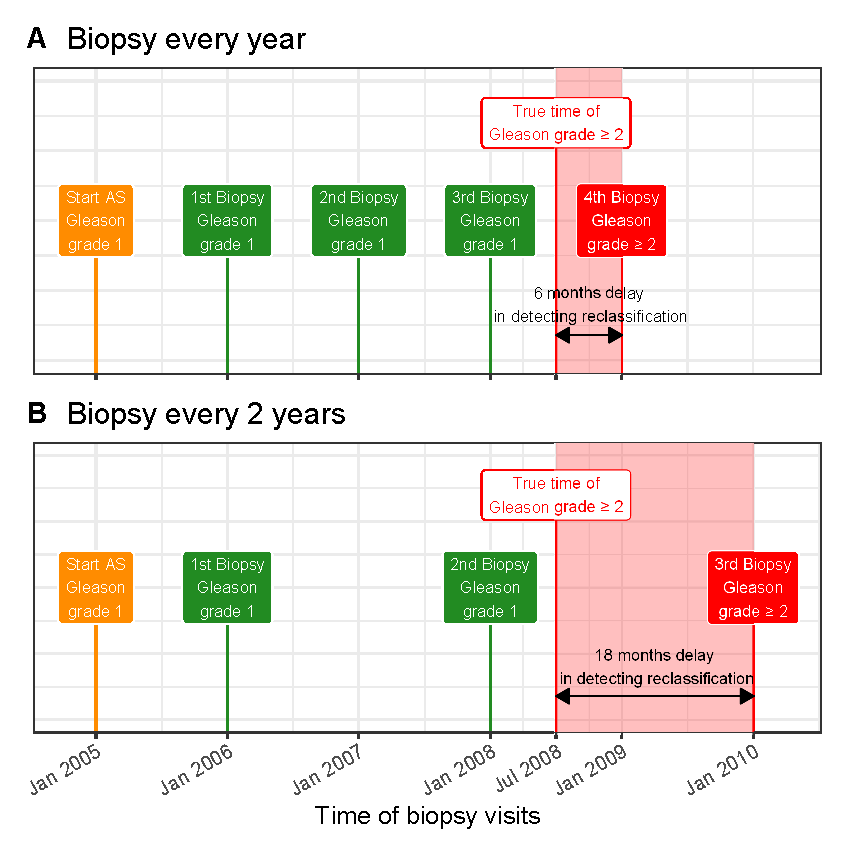
\includegraphics[width=\columnwidth]{images/delay_explanation.eps}}
\caption{\textbf{Trade-off between the number of biopsies and time delay in detecting reclassification (Increase in Gleason grade from 1 to 2 or higher):} The true time of reclassification for the patient in this figure is July 2008. When biopsies are scheduled annually (\textbf{Panel~A}), reclassification is detected in January 2009 with a time delay of six months, and a total of four biopsies are scheduled. When biopsies are scheduled biennially (\textbf{Panel~B}) reclassification is detected in January 2010 with a time delay of 18 months, and a total of three biopsies are scheduled. Since biopsies are conducted periodically, the time of reclassification is observed as an interval. For example, between Jan~2008--Jan~2009 in \textbf{Panel~A} and between Jan~2008--Jan~2010 in \textbf{Panel~B}.}
\label{fig:delay_explanation}
\end{figure}

Biopsies are conducted periodically. Consequently, reclassification is always detected with a time delay (Figure~\ref{fig:delay_explanation}). For detecting reclassification timely, many AS programs schedule fixed and frequent biopsies (e.g.,~annually) for all patients~\citep{nieboer2018active,loeb2014heterogeneity}. However, this also leads to many unnecessary biopsies in slow/non-progressing patients. Biopsies are invasive, painful and prone to medical complications. Thus, biopsy burden and patient non-compliance to frequent biopsies~\citep{bokhorst2015compliance} has raised concerns regarding the optimal biopsy schedule~\citep{inoue2018comparative, bratt2013study}. To this end, infrequent schedules such as biennial biopsies have been proposed as an alternative~\citep{inoue2018comparative,de2017estimating}. Although, biennial biopsies may still lead to five unnecessary biopsies over ten years (current study period of large AS programs) for slow/non-progressing patients. A promising alternative to fixed and frequent biopsies is personalized biopsy schedules based on the patient-specific risk of reclassification (Figure~\ref{fig:riskBasedExample}).

\begin{figure}
\centerline{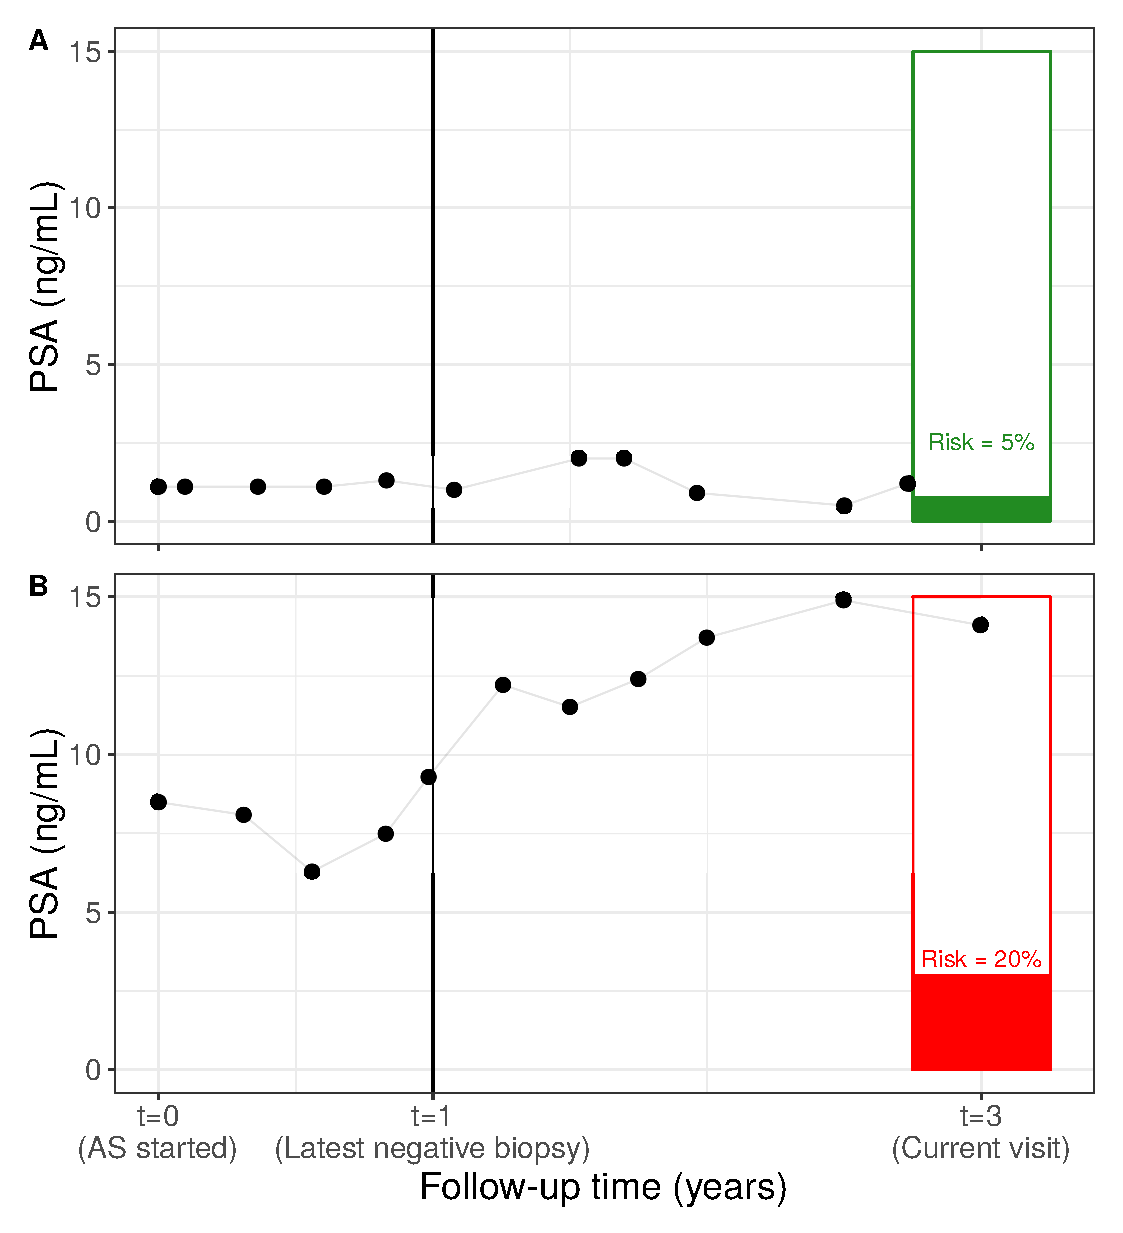
\includegraphics[width=\columnwidth]{images/riskBasedExample.eps}}
\caption{\textbf{Motivation for personalized risk-based decisions of biopsy}: Patient~A (\textbf{Panel~A}) and B (\textbf{Panel~B}) had their latest biopsy at year one of follow-up (green vertical line). Patient~A's prostate-specific antigen (PSA) profile remained stable until his current visit at year three, whereas patient~B's profile has shown a rise. Consequently, patient~B's estimated cumulative risk of reclassification at the current visit (year three) is higher than that of patient~A. This makes patient~B a more suitable candidate for biopsy than Patient~A. Risk estimates in this figure are only illustrative.}
\label{fig:riskBasedExample}
\end{figure}

The first challenge in developing personalized biopsy schedules is consolidating accumulated patient data (e.g., PSA, previous biopsy results) into risk estimates for reclassification. Existing calculators for risk of reclassification~\citep{partin1993use,makarov2007updated} use only the latest PSA measurement of a patient. In contrast, we intend to utilize all repeated measurements of PSA, previous biopsy results, and baseline characteristics of a patient. To this end, a suitable model is the joint model for time-to-event and longitudinal data~\citep{tomer2019, coley2017prediction,rizopoulos2012joint}. A joint model predicts risk of reclassification in a personalized manner. A subsequent challenge however, is translating risks into clinical decisions. For example, a 10\% risk of reclassification can be perceived high/low depending upon the patient age. Patients may also weigh risks of reclassification with the potential \textit{consequences} of another biopsy. Two relevant \textit{consequences} of biopsies (Figure~\ref{fig:delay_explanation}) are the timing and total number of biopsies (burden), and the time delay in detecting reclassification (smaller is beneficial). The relative importance of these \textit{consequences} can vary between the patients, and also over the follow-up period for the same patient.

The goal of this work was to assist patients and doctors in making better decisions of biopsies than fixed and frequent biopsies. For this purpose, we developed a web-application that gives patients their current and future risk of reclassification. It also suggests them risk-based personalized schedules of biopsies. For each biopsy schedule, be it fixed or personalized, the web-application provides expected \textit{consequences} of following it. Thus, patients can compare schedules before making a decision. The web-application uses a prediction joint model fitted to the world's largest AS dataset, PRIAS~\citep{bul2013active}. We externally validated this model in five largest AS cohorts of the GAP3 database \citep{gap3_2018}. Thus, the web-application can be used by a large number of patients worldwide.
% !TEX root =  ../main.tex 

\section{A framework for personalized biopsy schedules}
\label{sec : framework_pers_biop_sched}
The first step in creating a personalized schedule for biopsies is to come up with a model for Gleason scores, PSA levels and other patient specific characteristics. In PRIAS, PSA levels are measured at the time of induction, every 3 months for the first 2 years in the study and then every 6 months thereafter. Thus PSA levels can be modeled as a longitudinal outcome. As mentioned earlier, patients in PRIAS have a Gleason score of 6 or less at the time of induction in the study, and patients are removed from AS the first time GR takes place. Since our interest lies in finding the time of GR, we model it as a time to event outcome. While univariate modeling of the two aforementioned outcomes can be done separately using longitudinal model and survival models, but they are not independent. The association between the two exists because both are affected by the state of prostate cancer. To model the association between the two types of outcomes we use a joint model for time to event and longitudinal outcomes.

\subsection{Joint model for risk of GR and PSA levels}
\label{subsec : jm_definition}
Let $T_i^*$ denote the true GR time for the $i^{th}$ patient enrolled in an AS program. Let the vector of times at which a total of $g_i$ biopsies are conducted for the $i^{th}$ patient be denoted by $C_i = \{C_{i0}, C_{i1}, ... C_{ig_i}; C_{ij} < C_{ik}, \forall j<k \}$. $T_i^*$ cannot be observed directly and it is only known that it falls in an interval $(l_i, r_i]$, where $l_i = C_{i(g_i-1)}, r_i = C_{ig_i}$ if GR is observed, and $l_i = C_{ig_i}, r_i=\infty$ if patient drops out of AS. The latter is also known as right censoring. Let $\boldsymbol{y}_i$ denote the $n_i \times 1$ longitudinal outcome vector for the PSA levels of the $i^{th}$ patient. The population of interest is all the patients enrolled in AS. For a sample of $n$ patients from this population the complete data is denoted by $\mathcal{D}_n = \{T_i, l_i, r_i, \boldsymbol{y}_i; i = 1,...n\}$, where $T_i \epsilon (l_i, r_i]$ denotes the observed time of GR.\\

To model the evolution of the PSA measurements over time,  the joint model utilizes a linear mixed effects model. The longitudinal outcome $y_i(t)$ at a time $t$ is modeled as:

\begin{equation*}
\begin{split}
y_i(t) &= m_i(t) + \varepsilon_i(t), \\
&= \boldsymbol{x}_i^T(t) \boldsymbol{\beta} + \boldsymbol{z}_i^T(t) \boldsymbol{b}_i + \varepsilon_i(t)
\end{split}
\end{equation*}
%Do not introduce a space here, otherwise it starts a new paragraph
where, $m_i(t)$ denotes the true and unobserved value of the longitudinal outcome at time $t$. The measurement error $\varepsilon_i(t) \sim N(0, \sigma^2)$ is assumed normally distributed with variance $\sigma^2$. $\boldsymbol{\beta}$ denotes the vector of the unknown fixed-effects parameters. $\boldsymbol{b}_i \sim N(0, \boldsymbol{D})$ denotes the $q \times 1$ vector of random effects, assumed normally distributed with mean zero, and $q \times q$ covariance matrix $\boldsymbol{D}$. $\boldsymbol{b}_i$ and $\varepsilon_i(t)$ are assumed independent. $\boldsymbol{x}_i(t)$ and $\boldsymbol{z}_i(t)$ denote row vectors of the design matrices for the fixed and random effects, respectively. For non continuous longitudinal outcomes, joint models utilize Generalized linear mixed models \citep{rizopoulos2012joint}.\\

To model the effect of PSA measurements on risk of GR, joint models utilize a relative risk sub-model where the hazard of GR at any time point $t$, denoted by $h_i(t)$, depends on the history of true and unobserved values of PSA levels $\mathcal{M}_i(t) = \{m_i(v), 0\leq v \leq t\}$ measured up to that time point. Joint models offer flexibility in modeling this dependence. In its simplest form, the hazard may depend on instantaneous value of PSA $m_i(t)$ at time $t$. More sophisticated ones are dependence of hazard at time $t$ on PSA-DT, PSA velocity $m'_i(t) = \dfrac{d m_i(t)}{dt}$, or even on the cumulative effect of PSA $\int_0^t m_i(s) \,ds$ up to $t$. The fact that any functional form of dependence is possible, is evident from the following expression for hazard at time $t$:

\begin{equation*}
h_i(t \mid M_i(t), \boldsymbol{w}_i) = h_0(t) e^{\boldsymbol{\gamma}^T\boldsymbol{w}_i + f\{M_i(t), \boldsymbol{b}_i, \boldsymbol{\alpha}\}}
\end{equation*}
where $h_0(t)$ is the baseline hazard at time $t$. $\boldsymbol{w}_i$ is a vector of baseline covariates and $\boldsymbol{\gamma}$ are the corresponding parameters. The function $f(\cdot)$ parametrized by vector $\boldsymbol{\alpha}$ specifies the function form of longitudinal outcome that is used in the linear predictor of the relative risk model.\\

While $\boldsymbol{\alpha}$ controls the strength of association between the hazard of GR and features of the PSA history, the fact that both Gleason scores and PSA levels are internally related to a patient's health, is manifested by the random effects $\boldsymbol{b}_i$ in the model. The joint model postulates that given the random effects, time to GR and the different PSA measurements taken over time are all mutually independent. As mentioned earlier, in PRIAS study PSA-DT is used to decide the schedule of biopsies. Although PSA-DT is computed using observed PSA values, dependence on observed longitudinal history $\mathcal{Y}(t) = \{y_i(v), 0\leq v \leq t\}$ at any time $t$, is not the same as dependence on patient's health. On the contrary dependence on patient's health, manifested by $\boldsymbol{b}_i$ is same as dependence on future unobserved values of PSA. Thus the inference for the model parameters $\boldsymbol{\theta} = {\{\boldsymbol{\beta}^T, \boldsymbol{\gamma}^T, \boldsymbol{\alpha}^T, \sigma^2, \{d_{jk} \mid j=k=1,...q\}\}}^T$ doesn't change even if uncertainty in biopsy schedule $C_i$ is not modeled. The kernel of the corresponding joint likelihood conditional on the random effects and the model parameters is given by:

\begin{equation*}
p(T_i, l_i, r_i, \boldsymbol{y}_i \mid \boldsymbol{b}_i, \boldsymbol{\theta}) \propto p(T_i \mid l_i, r_i, \boldsymbol{b}_i, \boldsymbol{\theta}) p(\boldsymbol{y}_i \mid \boldsymbol{b}_i, \boldsymbol{\theta})
\end{equation*}

\subsection{Personalized scheduling approaches}
\label{subsec : pers_sched_approaches}
Once a joint model for GR and PSA levels is obtained, the next step is to use it to create personalized schedules for biopsies. In this section we present the various personalized biopsy scheduling approaches and their motivation. The personalized schedules that we propose are dynamic in nature and thus at any given time, only 1 future biopsy is scheduled. The age of the patient and entire PSA, repeat biopsy history up to that time point is considered while computing the time of next biopsy. To elucidate the scheduling methods, let us assume that the a personalized schedule is to be created a new patient enumerated $j$, who is not present in the original sample of patients $\mathcal{D}_n$. Further let us assume that this patient did not have a GR at their last biopsy performed at time $t$, and that the PSA measurements are available up to a time point $s$. Combining these two pieces of information, the predictive distribution $g(T^*_j)$ for time to GR for this patient is given by (conditioning on baseline covariates $\boldsymbol{w}_i$ is dropped for notational simplicity here onwards):

\begin{equation}
\label{eq : dyn_dist_fail_time}
\begin{split}
g(T^*_j) &= p(T^*_j \mid T^*_j > t, \mathcal{Y}_j(s), \mathcal{D}_n)\\
&= \int p(T^*_j \mid T^*_j > t, \mathcal{Y}_j(s), \boldsymbol{\theta}) p(\boldsymbol{\theta} \mid \mathcal{D}_n) \,d\boldsymbol{\theta}\\
&= \int \int p(T^*_j \mid T^*_j > t, \mathcal{Y}_j(s), \boldsymbol{b_j}, \boldsymbol{\theta}) p(\boldsymbol{b}_j \mid T^*_j>t, \mathcal{Y}_j(s), \boldsymbol{\theta})p(\boldsymbol{\theta} \mid \mathcal{D}_n) \,d\boldsymbol{b}_j \,d\boldsymbol{\theta}
\end{split}
\end{equation}
where $\mathcal{Y}_j(s)$ denotes the history of PSA measurements done up to time $s$. It can be seen that the predictive distribution depends on the observed longitudinal history via the random effects $\boldsymbol{b_j}$. The posterior distribution of the parameters $\boldsymbol{\theta}$ is obtained from the joint model fitted to the original data set of patients $\mathcal{D}_n$.\\

Given the predictive distribution $g(T^*_j)$, our goal is find the optimal time $u \geq \text{max}(t,s)$ of the next biopsy. To this end, we use principles from statistical decision theory in a Bayesian setting \citep{bergerDecisionTheory,robertBayesianChoice}. More specifically, we propose to choose future biopsy time $u$ by minimizing the posterior expected loss $E_g[L(T^*_j, u)]$, where the expectation is taken w.r.t. the predictive distribution $g(T^*_j)$. 

\begin{equation*}
E_g[L(T^*_j, u)] = \int_t^\infty L(T^*_j, u) p(T^*_j \mid T^*_j > t, \mathcal{Y}_j(s), \mathcal{D}_n) \,dT^*_j
\end{equation*}
Various loss functions $L(T^*_j, u)$ have been proposed in literature \citep{robertBayesianChoice}. The ones we utilize, and the corresponding motivations are presented next.

\subsubsection{Expected time of GR}
\label{subsubsec : exp_fail_time}
One of the reasons, patients did not comply with the existing PRIAS schedule was \textquoteleft complications on a previous biopsy \textquoteright. Therefore, it makes sense to have as less biopsies as possible. In the ideal case only 1 biopsy, performed at the exact time of GR is sufficient. Hence, neither a time which overshoots the true GR time $T^*_j$, nor a time which undershoots is preferred. In this regard, the squared loss function $L(T^*_j, u) = (T^*_j - u)^2$ and absolute loss function $L(T^*_j, u) = \mid T^*_j - u \mid$ have the properties that the posterior expected loss is symmetric on both sides of $T^*_j$. Secondly, both loss functions have well known solutions available. We first discuss the posterior expected loss for the squared loss function, given by:
%So the squared loss function satisfies our requirement of choosing a $u$ as close to the true GR time as possible. The is given by:
\begin{equation}
\label{eq : posterior_squared_loss}
\begin{split}
E_g[L(T^*_j, u)] &= E_g[(T^*_j - u)^2]\\
&=E_g[(T^*_j)^2] + u^2 -2uE_g[T^*_j]
\end{split}
\end{equation}
The posterior expected loss in equation \ref{eq : posterior_squared_loss} attains its minimum at $u = E_g[T^*_j]$, also known as expected time of GR.

\subsubsubsection{Estimation}
Since there is no closed form solution available for $E_g[T^*_j]$, for its estimation we introduce a construct called dynamic survival probability \citep{rizopoulos2011dynamic}. The dynamic survival probability $\pi_j(v \mid t, s)$ of patient $j$ is the survival probability at time $v$, conditional on the observed PSA history $\mathcal{Y}_j(s)$ and the fact that the patient did not have GR up to $t$. It is given by:

\begin{equation}
\pi_j(v \mid t, s) = Pr(T^*_j \geq v \mid  T^*_j >t, \mathcal{Y}_j(s), D_n), v \geq t
\end{equation}
The relationship between expected time of GR and dynamic survival probability is given by:

\begin{equation*}
E_g[T^*_j] = t + \int_t^\infty \pi_j(v \mid t, s) \,dv
\end{equation*}
Since the R package JMbayes already provides an implementation of $\pi_j(v \mid t, s)$, we preferred this approach over Monte Carlo methods to estimate $E_g[T^*_j]$ from the predictive distribution $g(T^*_j)$. There is no closed form solution available for the integral and hence we approximate it using Gauss-Kronrod quadrature. A limitation of \textquoteleft Expected time of GR though \textquoteright, is that it is practically useful only when the variance of predictive distribution $g(T^*_j)$ is small. The variance is given by:

\begin{equation}
\begin{split}
Var_g[T^*_j] &= E_g[{T^*_j}^2] - {E_g[T^*_j]}^2\\
&= 2 \int_t^\infty {(v-t) \pi_j(v \mid t, s) \,dv} - {\bigg(\int_t^\infty \pi_j(v \mid t, s) \,dv\bigg)}^2
\end{split}
\end{equation}
Once again, a closed form solution is not available for the variance expression. The variance however depends on both $t$ and $\mathcal{Y}_j(s)$. To elucidate the relationship between variance and observed information, we computed the variance at different time points for a couple of patients from the PRIAS study. The corresponding joint model fitted to the data set is discussed in section \ref{subsec : jm_fit_prias}. The first patient in question is patient nr. 405. He visited the hospital 53 times and was then right censored. 5 out those 53 visits were for biopsies. The variance of predictive distribution after each of those visits is shown in Figure \ref{fig : variance_pred_dist}. It is clear that the variance drops by a large margin each time a biopsy is conducted. i.e. when more information about $T^*_j$ is available. The effect of $\mathcal{Y}_j(s)$ on variance can be seen in Figure \ref{fig : variance_pred_dist_3174} which corresponds to patient nr. 3174, who visited the hospital 9 times and was censored after his last biopsy. The observed PSA measurements for this patient are shown in Figure \ref{fig : observed_psa_3174}. It can be seen that the variance doesn't depend on number of PSA measurements, but rather on the measurement values. For patient nr. 3174, variance drops quickly when PSA measurements increase sharply.  This becomes intuitive when we look at the model parameter estimates (section \ref{subsec : param_estimates_jm_fit_prias}), where rate of change of PSA $m'_i(t)$ is a strong predictor of the hazard of GR.

\begin{figure}[!htb]
    \centering
    \captionsetup{justification=centering}
    \begin{subfigure}[b]{0.45\textwidth}
        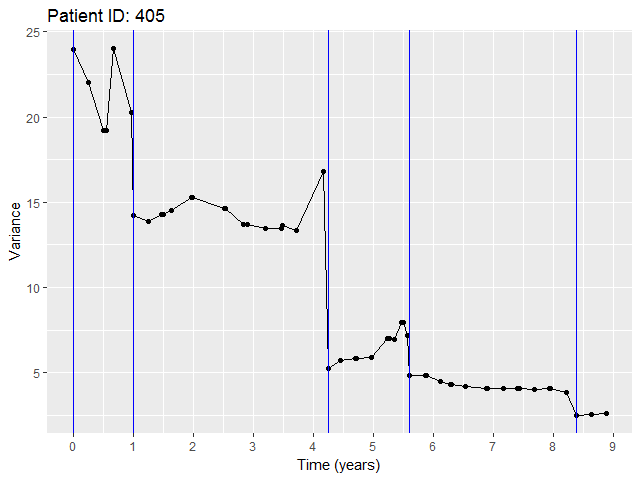
\includegraphics[width=\textwidth]{images/variance_pred_dist_405.png}
        \caption{Variance of the predictive distribution $g(T^*_j)$ over a period of 9 years for patient 405. Blue vertical lines indicate biopsies.}
        \label{fig : variance_pred_dist_405}
    \end{subfigure}   
    \begin{subfigure}[b]{0.45\textwidth}
        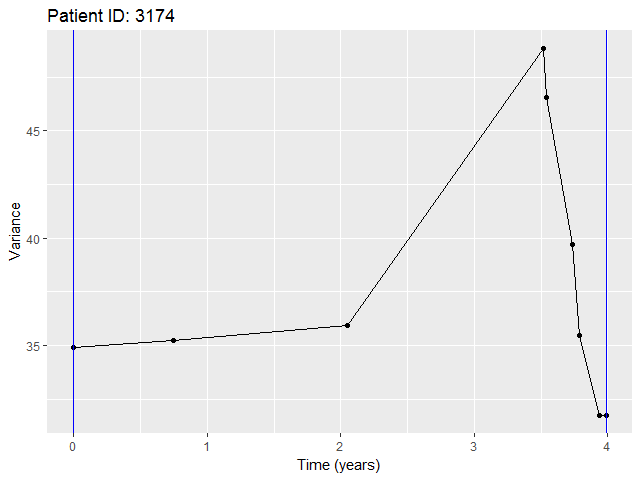
\includegraphics[width=\textwidth]{images/variance_pred_dist_3174.png}
        \caption{Variance of the predictive distribution $g(T^*_j)$ over a period of 4 years for patient 405. Blue vertical lines indicate biopsies.}
        \label{fig : variance_pred_dist_3174}
    \end{subfigure}
    \caption{Variance of the predictive distribution $g(T^*_j)$}\label{fig : variance_pred_dist}
\end{figure}

\begin{figure}[!htb]
    \centering
    \captionsetup{justification=centering}
    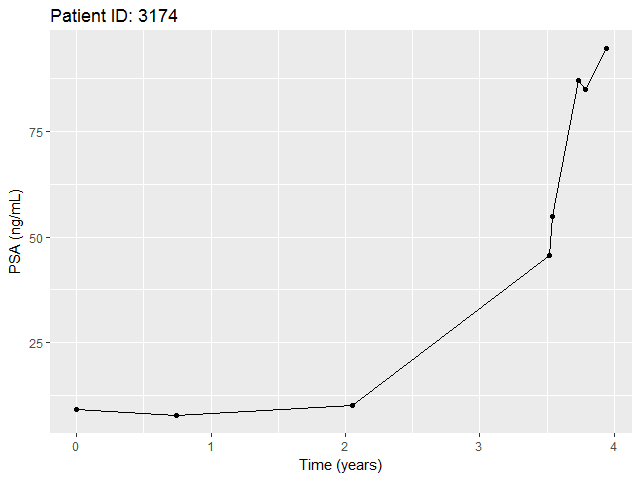
\includegraphics[width=0.5\textwidth]{images/observed_psa_3174.png}
    \caption{Observed evolution of PSA for patient 3174.}
    \label{fig : observed_psa_3174}
\end{figure}

\subsubsection{Dynamic risk of GR}
\label{subsubsec : dynamic_risk_definitions}
In a practical scenario it is possible that a doctor or a patient may not want to exceed a certain risk of GR $1 - \pi_j(u \mid t, s)$ since the last biopsy. This may be also useful in the cases where variance of $g(T^*_j)$ is high, rendering expected time of GR unsuitable. The personalized scheduling approach based on dynamic risk of GR, schedules the next biopsy at a time point $u$ such that the dynamic risk of GR is higher than a certain threshold $1-\kappa,\ \kappa \epsilon [0,1]$ beyond $u$. Or in other words the dynamic survival probability $\pi_j(u \mid t, s)$ is below a threshold $\kappa$ beyond $u$. In this regard, the posterior expected loss for the following multilinear loss function can be minimized to find the most optimal $u$:

\begin{equation}
\label{eq : loss_dynamic_risk}
L_{k_1, k_2}(T^*_j, u) =
    \begin{cases}
      k_2(T^*_j-u) & if(T^*_j > u)\\
      k_1(u-T^*_j) & \text{otherwise}
    \end{cases}       
\end{equation}
where $k_1 > 0$, $k_2 > 0$ are constants parameterizing the loss function. The posterior expected loss function $E_g[L_{k_1, k_2}(T^*_j, u)]$ obtains its minimum at $u = \pi_j^{-1}\Big\{\dfrac{k_1}{k_1 + k_2}\Big\}$ \citep{robertBayesianChoice}. The choice of $k_1, k_2$ is equivalent to the choice of $\kappa$. More specifically, $\kappa = \dfrac{k_1}{k_1 + k_2}$. When $k_1=k_2=1$, the multilinear loss function is equal to the absolute loss function $L(T^*_j, u) = \mid T^*_j - u \mid$. Since $\kappa = 0.5$ for absolute loss, time $u$ is the median of the predictive distribution $g(T^*_j)$.

\subsubsubsection{Choice of $\kappa$}
Since the value $\kappa$ dictates the biopsy schedule, its choice has important consequences. In certain cases it may be chosen on the basis of doctor's advice or the amount of risk that is acceptable to the patient. For e.g. if maximum acceptable risk is 75\% then $\kappa = 0.25$ and correspondingly, all $k_1, k_2 \mid k_1=\dfrac{k_2}{3}$ can be used in equation \ref{eq : loss_dynamic_risk} to calculate $u$. \\

While expert advice can be invaluable, it is also possible to automate the choice of $\kappa$. We propose to choose a $\kappa$ for which a binary classification accuracy measure \citep{lopez2014optimalcutpoints,sokolova2009systematic}, discriminating between cases and controls, is maximized. In PRIAS, cases are patients who experience GR and the rest are controls. However, a patient can be in control group at some time $t_a$ and in the cases at some future time point $t_b > t_a$, and thus time dependent binary classification is more relevant. In joint models, a patient $j$ is predicted to be a case if $\pi_j(t + \Delta t \mid t,s) \leq \kappa$ and a control if $\pi_j(t + \Delta t \mid t,s) > \kappa$ \citep{rizopoulosJMbayes}. The time window $\Delta t$ can be either chosen on a clinical basis (such as 1 year in PRIAS \textcolor{red}{\textbf{WHY 1 YEAR}}) or it can be chosen at a point where $AUC(t, \Delta t, s)$ \citep{rizopoulosJMbayes} is largest. i.e. $\Delta t$ for which the model has the most discriminative capability at time $t$. The binary classification accuracy measures we maximize to select the threshold $\kappa$ are the following (the binary classification measures are functions of $t, \Delta t, s$, although the notation is dropped for readability): 

\begin{itemize}
\item Accuracy: $ACC = \dfrac{TP + TN}{TP + FP + TN + FN}$, where TP, FP, TN and FN are the number of true positives, false positives, true negatives and false negatives at time point $t$. In this case if $k_1 = TP + TN$ and $k_2 = FP + FN$, then $\argmax{k_1, k_2} ACC$ gives the optimal $k_1, k_2$ or equivalently the $\kappa$.

\item Youden's index: $J = \text{Sensitivity} + \text{Specificity}- 1$,\\
where sensitivity is defined as $Pr(\pi_j(t + \Delta t \mid t,s) \leq \kappa \mid T^*_j \epsilon (t, t + \Delta t])$ and specificity is defined as $Pr(\pi_j(t + \Delta t \mid t,s) > \kappa \mid T^*_j > t + \Delta t)$. In this case if $k_1 = FP \cdot TP - FN \cdot TN$ and $k_2 = (TP+FN)(FP+TN) - k_1$, then $\argmax{k_1, k_2} J$ gives the optimal $k_1, k_2$ or equivalently the $\kappa$.

\item F1 Score: $F1 = \dfrac{2TP}{2TP + FP + FN}$. In this case if $k_1 = 2TP$ and $k_2 = FP + FN$, then $\argmax{k_1, k_2} F1$ gives the optimal $k_1, k_2$ or equivalently the $\kappa$.
\end{itemize}

\subsubsection{Mixed approach}

\subsubsection{Scheduling multiple biopsies}
\label{subsubsec : pers_sched_algorithm}
Scheduling biopsies using personalized schedules is an iterative process. Only one biopsy is scheduled at once, using all the information available up to that point in time. The information is manifested via the predictive distribution $g(T^*_j)$. It is important to note that new biopsy times are only proposed when the patient visits the hospital for a PSA measurement or for biopsy, since $g(T^*_j)$ is updated only at these time points. If a biopsy is conducted at time $t$, then scheduling the next biopsy at time $u \geq \text{max}(t,s)$ for patient $j$ is the goal. Although the predictive distribution $g(T^*_j)$ is updated with the new information $T^*_j > t$, there are a couple of restrictions on time $u$, namely:

\begin{enumerate}
\item Two consecutive biopsies should have a gap of at least 1 year between them. i.e. $u \geq t + 1$. Given the medical side effects of biopsies, the 1 year gap is strongly advised for patients enrolled in PRIAS. However, the personalized scheduling methods do not take this rule into account.
\item Although it is required that $u \geq \text{max}(t,s)$, the personalized scheduling methods may propose to perform a biopsy at a time $u \epsilon (t, s]$. The reason is that, GR is not a terminating event, and so the patients continue to visit for PSA measurements. The support of the predictive distribution $g(T^*_j)$, however does not depend on last time of PSA measurement $s$, and remains $(t, \infty)$.
\end{enumerate}
 
Lastly, it is extremely likely that on consecutive visits to the hospital for PSA measurements, the personalized biopsy time is postponed or preponed. The choice of time of biopsy from consecutive visits is not clear. To resolve these issues, we propose to supplement the personalized scheduling methods with the following algorithm.

\subsubsubsection{Algorithm}
Let us assume that patient $j$ had their latest biopsy at time $T^l_j$, and the latest available PSA measurement is from the current visit to the hospital, at time $T^{cv}_j$. The predictive distribution for time of GR is given by $p(T^*_j|T^*_j > T^l_j, \mathcal{Y}_j(T^{cv}_j), \mathcal{D}_n)$. Further let,

\begin{enumerate}
\item $T^p_j$ denote the time at which a biopsy is proposed by personalized scheduling methods.
\item Let $T^s_j$ denote the time at which a biopsy is scheduled. This is not necessarily equal to the proposed time $T^p_j$, but rather a time devoid of the problems mentioned earlier. This time is generated from the algorithm.
\item $T^{nv}_j$ denote the time of the next visit for PSA.
\item $N^b_j$ denote the counter for number of biopsies conducted up to time $T^l_j$, excluding the biopsy done at the time of induction in AS.
\end{enumerate}
Using these constructs, we have proposed an algorithm to schedule multiple biopsies. It is shown in Figure \ref{fig : sched_algorithm}. 

\begin{figure}[!htb]
\centering
\captionsetup{justification=centering}
\resizebox{0.65\columnwidth}{!}{%

\begin{tikzpicture}
\node (start) [startstop] {
Enter Active Surveillance.
\begin{enumerate}
\item Conduct a biopsy.
\item Set $t=T^{nv}=0$ 
\item Set $u = \infty$
\end{enumerate}
};

\node (takePSA) [process_wide_5cm, below=1cm of start] {
\begin{enumerate}
\item Measure PSA at $T^{nv}$ 
\item Set $s=T^{nv}$
\end{enumerate}
};

\node (propTime) [process_wide_3pt5cm, below=1cm of takePSA] {
\begin{enumerate}
\item Set $u^{pv} = u$ 
\item Update $g(T^*_j)$ 
\item Propose $u$
\end{enumerate}
};

\node (decision1) [decision, below = 1.5cm of propTime] {$u < u^{pv}$};
\node (pro6) [process, right = 1.35cm of decision1] {Set $u = u^{pv}$};

\node (decision5) [decision, left=1.5cm of decision1] {$u \leq s$};

\node (pro5) [process, below=1.5cm of decision5] {Set $u = s$};

\node (decision2) [decision, below=0.5cm of decision1] {$u - t > 1$};

\node (decision4) [decision, right=1.5cm of decision2] {$u > T^{nv}$};

\node (pro3) [process_wide_3pt5cm, below=1cm of decision2] {
\begin{enumerate}
\item Conduct Biopsy at $t + 1$ 
\item Set $t = t + 1$
\end{enumerate}
};

\node (pro4) [process_wide_3pt5cm, below=1cm of decision4] {
\begin{enumerate}
\item Conduct Biopsy at $u$
\item Set $t = u$
\end{enumerate}
};

\node (decision3) [decision, below=1cm of pro3] {$\mbox{Gleason} > 6$};
\node (pro7) [process, left=1cm of decision3] {Set $u=\infty$};

\node (stop) [startstop, below = 1cm of decision3] {Remove patient from AS};

\draw [arrow] (start) -- (takePSA);
\draw [arrow] (takePSA) -- (propTime);
\draw [arrow] (propTime) -- (decision1);
\draw [arrow] (decision1) -- node[anchor=south] {Yes} (decision5);
\draw [arrow] (decision5) -- node[anchor=east] {Yes} (pro5);
\draw [arrow] (pro5) -- (decision2);
\draw [arrow] (decision1) -- node[anchor=south] {No} (pro6);
\draw [arrow] (decision5) -- node[anchor=south] {No} (decision2);
\draw [arrow] (pro6) -- (decision4);
\draw [arrow] (decision4.east) |- ([xshift=0.35cm, yshift=-4.15cm]pro6.north east) |- node[anchor=south] {Yes} (takePSA);
\draw [arrow] (decision2) -- node[anchor=south] {Yes} (decision4);
\draw [arrow] (decision2) -- node[anchor=east] {No} (pro3);
\draw [arrow] (pro3) -- (decision3);
\draw [arrow] (pro4) |- (decision3);
\draw [arrow] (decision3) -- node[anchor=east] {Yes} (stop);
\draw [arrow] (decision4) -- node[anchor=east] {No} (pro4);
\draw [arrow] (decision3) -- node[anchor=south]{No} (pro7);
\draw [arrow] (pro7.west)|- ([xshift=-0.35cm, yshift=-7.8cm]pro5.north west) |- (propTime);
\end{tikzpicture}

}%


\caption{Algorithm for scheduling multiple biopsies using personalized schedules.} 
\label{fig : sched_algorithm}
\end{figure}
% !TEX root =  ../main.tex 

\section{Personalized schedules for patients in PRIAS}
\label{sec : pers_schedule_PRIAS}
As a first step in demonstrating how the personalized schedules work, we created a biopsy schedule for patients in PRIAS. To this end, we divided the PRIAS data set into training(5938 subjects) and demonstration data sets (5 subjects). We demonstrate that the biopsy schedule depend on subject specific traits and the evolution of PSA scores.\\ 

\begin{figure}[!htb]
\centering
\captionsetup{justification=centering}
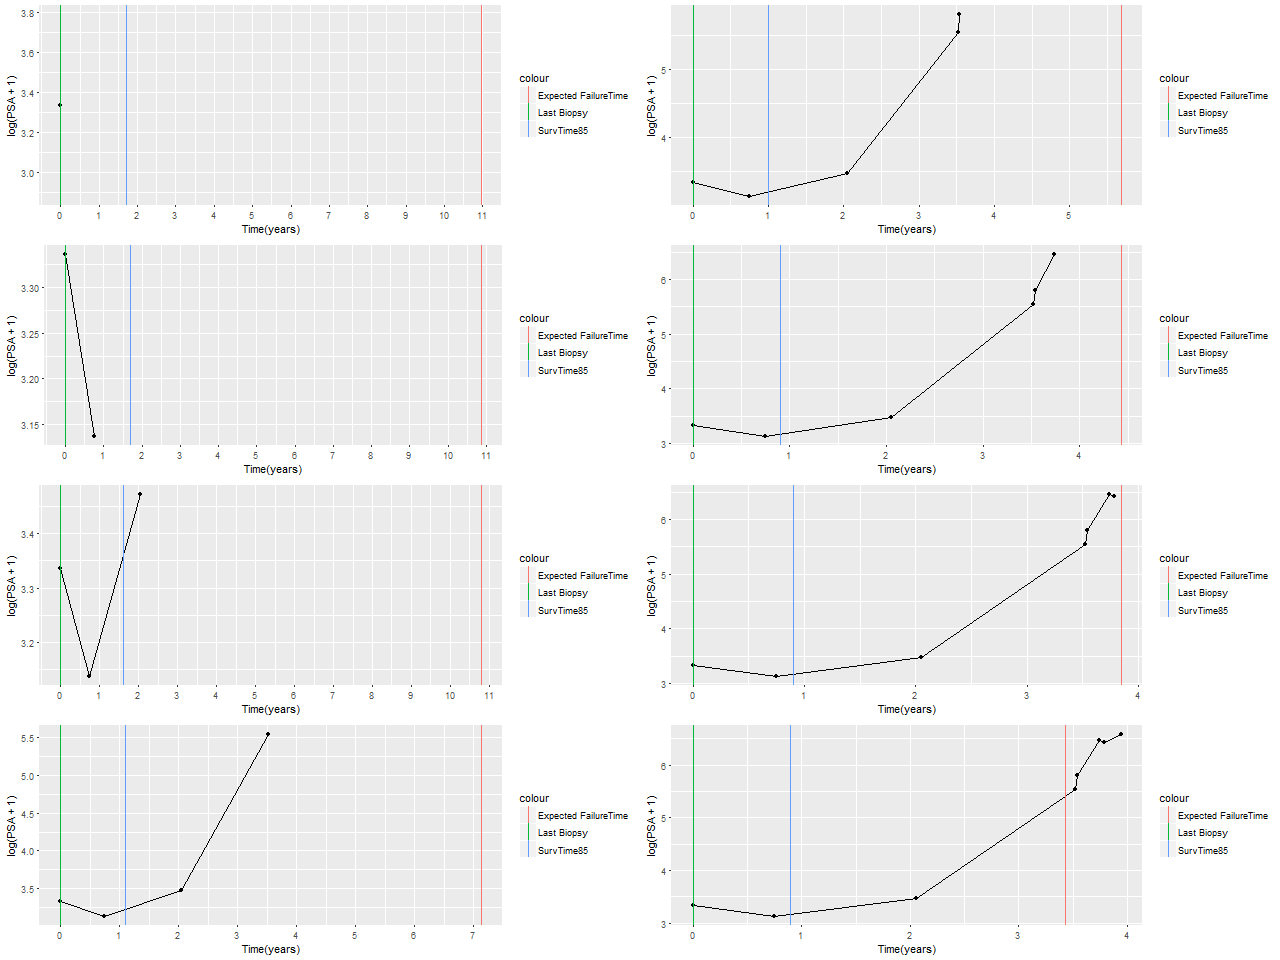
\includegraphics[width=\textwidth]{prias_demo_pid_3174.png}
\caption{\label{fig : prias_demo_pid_3174} Proposed biopsy times for patient 3174 from PRIAS.}
\end{figure}

\begin{figure}[!htb]
\centering
\captionsetup{justification=centering}
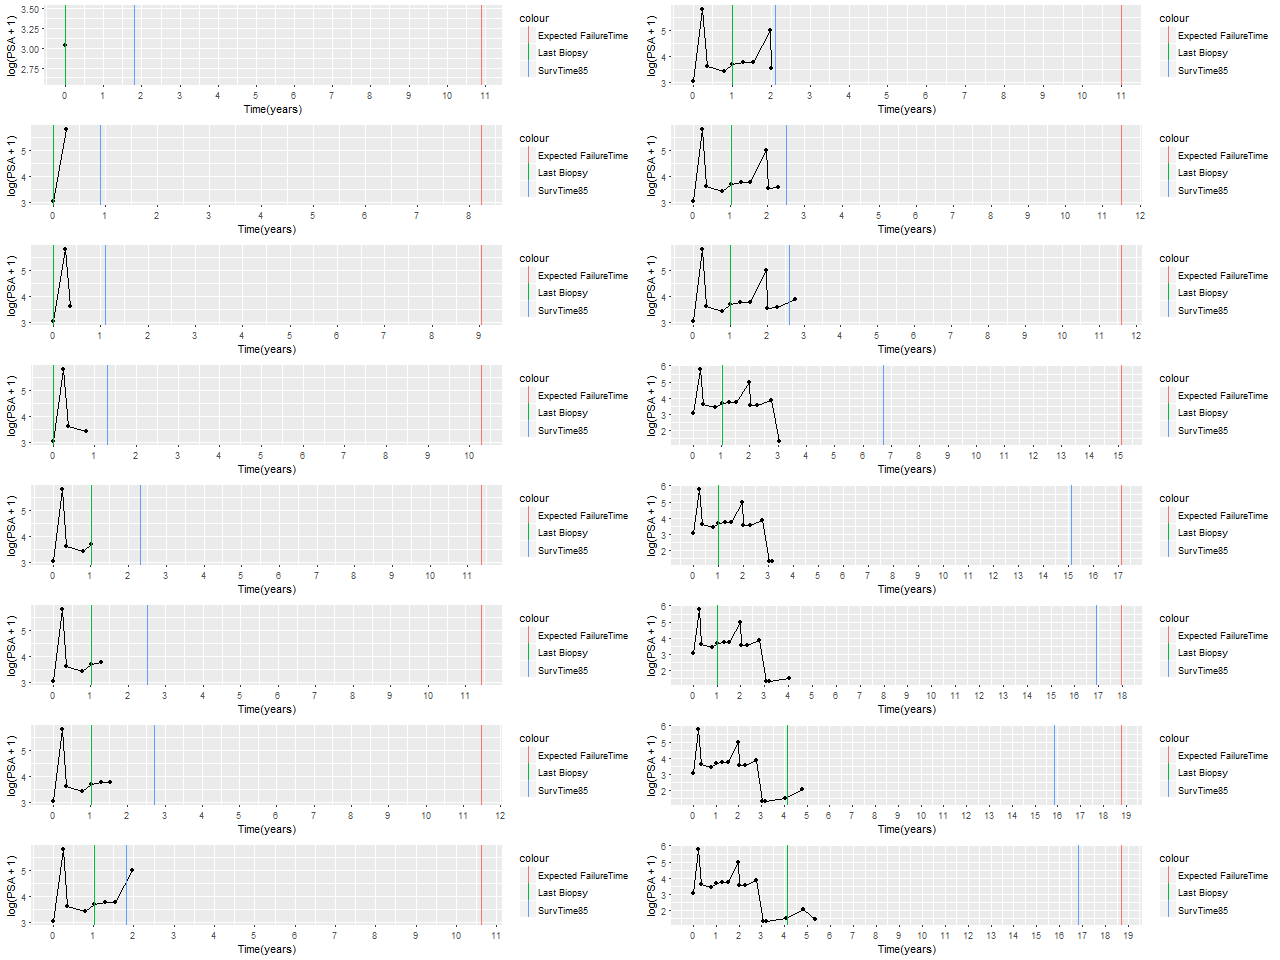
\includegraphics[width=\textwidth]{prias_demo_pid_911.png}
\caption{\label{fig : prias_demo_pid_911} Proposed biopsy times for patient 3174 from PRIAS.}
\end{figure}

\begin{figure}[!htb]
\centering
\captionsetup{justification=centering}
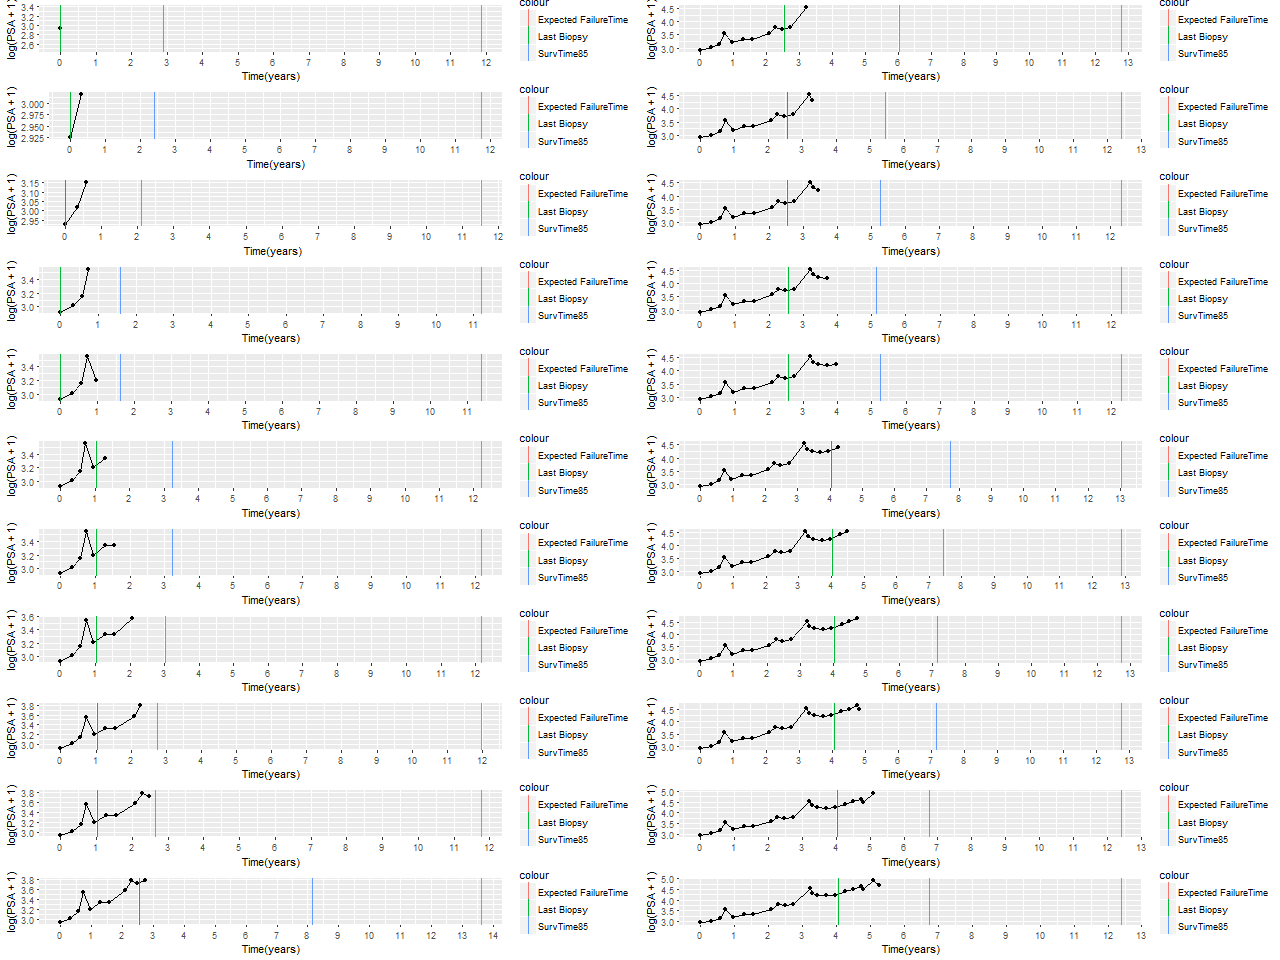
\includegraphics[width=\textwidth]{prias_demo_pid_2340.png}
\caption{\label{fig : prias_demo_pid_2340} Proposed biopsy times for patient 3174 from PRIAS.}
\end{figure}

It can be seen in Figure \ref{fig : prias_demo_pid_3174} that the patient 3174 had a biopsy at the time of induction and none after that. The PSA for the patient increases rapidly after the 2nd year. In response to this rapid increase, the proposed biopsy times based on conditional expected failure time also decrease accordingly from 11 years to around 3.4 years. The change for risk based methods is not so drastic though. Further it can be seen that at the last visit for PSA, the proposed biopsy time is earlier than the last 5 PSA visits and similar is the case for the proposed biopsy time based on dynamic risk of failure. This is due to the fact that the last time of biopsy was time 0 (induction time) and thus the time to Gleason reclassification can take any value larger than 0. We discuss this issue in detail in section \ref{subsec : simulation_setup}.\\

Figure \ref{fig : prias_demo_pid_911} shows the PSA evolution and biopsy times for subject 911. It can be seen that this patient had 3 biopsies where Gleason reclassification did not happen. At year 2 when the patient's PSA increases rapidly the proposed failure times also decrease, whereas they increase over the next 1 year because the PSA also drops down in that time period. The fact that PSA velocity affects the biopsy times the most is also evident in the case of subject 2340, whose evolution is shown in Figure \ref{fig : prias_demo_pid_2340}. Here the rate of change at each time point is not high, and even though the PSA value reaches as high as 25 it has no effect on proposed biopsy times. This is in accordance with the estimated strength of association between PSA velocity/value and hazard of time to Gleason reclassification.\\

An interesting observation we made while creating these schedules was that the variance of time to Gleason reclassification (Eq. \ref{eq : varFailureTime}) was quite high, which essentially rules out the usefulness of conditional expected time to Gleason reclassification. Given the large difference in proposed biopsy times based on the former and methods based on dynamic risk of Gleason reclassification, one might conclude that the latter are more useful. However as we will see in the simulation study (Section \ref{sec: simulation_study}) ahead, the usefulness of the two categories of methods depends on the distribution of time to Gleason reclassification.

% !TEX root =  ../main_manuscript.tex 
\section{Simulation Study}
\label{sec: simulation_study}
In Section \ref{subsec : demo_prias_pers_schedule} we demonstrated that the personalized schedules, schedule future biopsies according to the historical data of each patient. However, we could not perform a full-scale comparison between personalized and PRIAS schedules, because the true time of GR was not known for the PRIAS patients. To this end, we conducted a simulation study comparing personalized schedules with PRIAS and annual schedule, whose details are presented next.

\subsection{Simulation Setup}
\label{subsec : simulation_setup}
The population of AS patients in this simulation study is assumed to have the same entrance criteria as that of PRIAS. The PSA and hazard of GR for these patients follow a joint model of the form postulated in Section \ref{subsec : jm_fit_prias}, with parameters equal to the posterior mean of parameters estimated from the joint model fitted to the PRIAS dataset (see Web Appendix C). Furthermore, we also intend to test the efficacy of different schedules for a population which has patients with both faster as well as slowly-progressing PCa. The rate of progression is not only manifested via PSA profiles but also via the baseline hazard. We assume that there are three equal sized subgroups $G_1$, $G_2$ and $G_3$ of patients in the population, each with a baseline hazard from a Weibull distribution, with the following shape and scale parameters $(k, \lambda$): $(1.5, 4)$, $(3, 5)$ and $(4.5, 6)$ for $G_1, G_2$ and $G_3$, respectively. The effect of these parameters is that the mean GR time is lowest in $G_1$ (fast PCa progression) and highest in $G_3$ (slow PCa progression).

From this population, we have sampled 500 datasets with 1000 patients each. We generate a true GR time for each of the patients, and then sample a set of PSA measurements at the same time points as given in PRIAS protocol (see Web Appendix C). We then split the dataset into a training (750 patients) and a test (250 patients) part, and generate a random and non-informative censoring time for the training patients. We next fit a joint model of the specification given in (\ref{eq : long_model_prias}) and (\ref{eq : hazard_prias}) to each of the 500 training datasets and obtain MCMC samples from the 500 sets of the posterior distribution of the parameters. Using these fitted joint models, we obtain the posterior predictive distribution of time of GR for each of the $500 \times 250$ test patients. This distribution is further used to create personalized biopsy schedules for the test patients. For every test patient we conduct hypothetical biopsies using the following six types of schedules (abbreviated names in parenthesis): personalized schedules based on expected time of GR (Exp. GR time) and median time of GR (Med. GR time), personalized schedules based on dynamic risk of GR (Dyn. risk GR), a hybrid approach between median time of GR and dynamic risk of GR (Hybrid), PRIAS schedule and the annual schedule. The biopsies are conducted as per the algorithm in Figure \ref{fig : sched_algorithm}. 

To compare the aforementioned schedules we require estimates of the various measures of efficacy described in Section \ref{sec : choosing_schedule}. To this end, for schedule $S$, we compute pooled estimates of mean offset $E(O^S_j)$ and variance of offset $\mbox{var}(O^S_j)$, as below (estimates for $N^S_j$ are similar):
\begin{align*}
\widehat{E(O^S_j)} &= \frac{\sum_{k=1}^{500} n_k \widehat{E(O^S_k)}}{\sum_{k=1}^{500} n_k}, \\
\widehat{\mbox{var}(O^S_j)} &= \frac{\sum_{k=1}^{500} (n_k - 1) \widehat{\mbox{var}(O^S_k)}}{\sum_{k=1}^{500} (n_k-1)}, 
\end{align*}
where $n_k$ denotes the number of test patients, $\widehat{E(O^S_k)} = {\sum_{l=1}^{n_k}O^S_{kl}}/{n_k}$ is the estimated mean and $\widehat{\mbox{var}(O^S_k)} = {\sum_{l=1}^{n_k}\big\{O^S_{kl} - \widehat{E(O^S_k)}\big\}^2}/(n_k-1)$ is the estimated variance of the offset for the $k$-th simulation. The offset for the $l$-th test patient of the $k$-th dataset is denoted by $O^S_{kl}$.

\subsection{Results}
The pooled estimates of the aforementioned measures are summarized in Table \ref{table : sim_study_pooled_estimates}. In addition, estimated values of $E(O^S_j)$ are plotted against $E(N^S_j)$ in Figure \ref{fig : meanNbVsOffset}. The figure shows that across the schedules there is an inverse relationship between number $E(O^S_j)$ and $E(N^S_j)$. For example, the annual schedule conducts on average 5.2 biopsies to detect GR, which is the highest among all schedules. However, it has the least average offset of 6 months as well. On the other hand, the schedule based on expected time of GR conducts only 1.9 biopsies on average to detect GR, the least among all schedules, but it also has the highest average offset of 15 months (similar for median time of GR). Since the annual schedule attempts to contain the offset within a year it has the least $\mbox{SD}(O^S_j) = \sqrt{\mbox{var}(O^S_j)}$. However to achieve this, it conducts a wide range of number of biopsies from patient to patient, i.e., highest $\mbox{SD}(N^S_j) = \sqrt{\mbox{var}(N^S_j)}$. In this regard, schedules based on expected and median time of GR perform the opposite of annual schedule.

\begin{figure}
\centerline{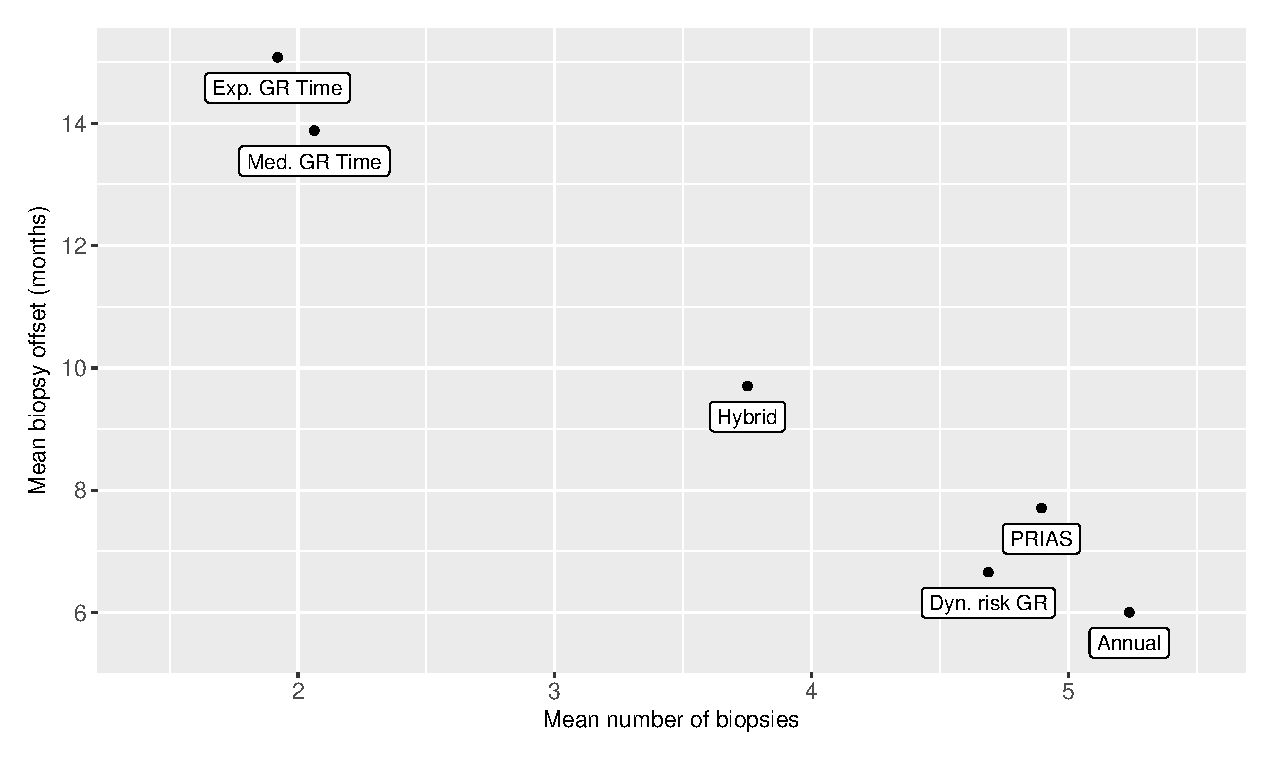
\includegraphics[width=\columnwidth]{images/sim_study/meanNbVsOffset_all.eps}}
\caption{Estimated mean number of biopsies and mean offset (months) for various schedules, obtained from the simulation study with 500 simulated datasets.}
\label{fig : meanNbVsOffset}
\end{figure}

%124781 = 41484 + 41423 + 41874
\begin{table}
\caption{Estimated mean and standard deviation of the number of biopsies $N^S_j$ and offset $O^S_j$ (months) for various schedules, obtained from the simulation study with 500 simulated datasets.}
\label{table : sim_study_pooled_estimates}
\begin{tabular}{lrrrr}
\Hline
\multicolumn{5}{c}{a) All hypothetical subgroups}\\
\hline
Schedule          & $E(N^S_j)$ & $E(O^S_j)$ & ${\mbox{SD}(N^S_j)}$ & ${\mbox{SD}(O^S_j)}$ \\
\hline
Annual         & 5.24            & 6.01                & 2.53          & 3.46              \\
PRIAS          & 4.90            & 7.71                & 2.36          & 6.31\\
Dyn. risk GR       & 4.69            & 6.66                & 2.19           & 4.38              \\
Hybrid       & 3.75            & 9.70                & 1.71          & 7.25              \\
Med. GR time & 2.06            & 13.88               & 1.41          & 11.80              \\
Exp. GR time & 1.92            & 15.08               & 1.19          & 12.11             \\
\hline
\multicolumn{5}{c}{b) Hypothetical subgroup $G_1$}\\
\hline
Schedule        & $E(N^S_j)$ & $E(O^S_j)$ & ${\mbox{SD}(N^S_j)}$ & ${\mbox{SD}(O^S_j)}$ \\
\hline
Annual         & 4.32            & 6.02                & 3.13          & 3.44              \\
PRIAS          & 4.07            & 7.44                & 2.88          & 6.11    \\
Dyn. risk GR       & 3.85            & 6.75                & 2.69          & 4.44              \\
Hybrid       & 3.25            & 10.25               & 2.16          & 8.07              \\
Med. GR time & 1.84            & 20.66               & 1.76          & 14.62             \\
Exp. GR time & 1.72            & 21.65               & 1.47          & 14.75             \\
\hline      
\multicolumn{5}{c}{c) Hypothetical subgroup $G_2$}\\
\hline
Schedule        & $E(N^S_j)$ & $E(O^S_j)$ & ${\mbox{SD}(N^S_j)}$ & ${\mbox{SD}(O^S_j)}$ \\
\hline
Annual         & 5.18            & 5.98                & 2.13          & 3.47              \\
PRIAS          & 4.85            & 7.70                & 2.00          & 6.29        \\
Dyn. risk GR       & 4.63            & 6.66                & 1.82          & 4.37              \\
Hybrid       & 3.68            & 10.32                & 1.37          & 7.45              \\
Med. GR time & 1.89             & 12.33               & 1.16          & 9.44              \\
Exp. GR time & 1.77            & 13.54               & 0.98          & 9.83              \\
\hline      
\multicolumn{5}{c}{d) Hypothetical subgroup $G_3$}\\
\hline
Schedule        & $E(N^S_j)$ & $E(O^S_j)$ & ${\mbox{SD}(N^S_j)}$ & ${\mbox{SD}(O^S_j)}$ \\
\hline
Annual         & 6.20             & 6.02                & 1.76          & 3.46              \\
PRIAS          & 5.76             & 7.98                & 1.71         & 6.51        \\
Dyn. risk GR       & 5.58            & 6.58                & 1.56          & 4.33              \\
Hybrid       & 4.32            & 8.55                & 1.26          & 5.91              \\
Med. GR time & 2.45            & 8.70                & 1.15          & 6.32              \\
Exp. GR time & 2.27            & 10.09               & 0.99          & 7.47              \\
\hline     
\end{tabular}
\end{table}

The PRIAS schedule conducts only 0.3 biopsies less than the annual schedule, but with a higher $\mbox{SD}(O^S_j)$, early detection is not always guaranteed. In comparison, the dynamic risk of GR based schedule performs slightly better than the PRIAS schedule in all four criteria. The hybrid approach combines the benefits of methods with low $E(N^S_j)$ and $\mbox{SD}(N^S_j)$, and methods with low $E(O^S_j)$ and $\mbox{SD}(O^S_j)$. It conducts 1.5 biopsies less than the annual schedule on average and with a $E(O^S_j)$ of 9.7 months it detects GR within a year since its occurrence. Moreover, it has both $\mbox{SD}(N^S_j)$ and $\mbox{SD}(O^S_j)$ comparable to PRIAS.

The performance of each schedule differs for the three subgroups $G_1, G_2$ and $G_3$. The annual schedule remains the most consistent across subgroups in terms of the offset, but it conducts 2 extra biopsies for the subgroup $G_3$ (slowly-progressing PCa) than $G_1$ (faster-progressing PCa). The performance of schedule based on expected time of GR is the most consistent in terms of the number of biopsies but it detects GR a year later on average in subgroup $G_1$ than $G_3$. For the dynamic risk of GR based schedule and the hybrid schedule, the dynamics are similar to that of the annual schedule. Unlike the latter two schedules, the PRIAS schedule not only conducts more biopsies in $G_3$ than $G_1$ but also detects GR later in $G_3$ than $G_1$.

\begin{figure}[!htb]
\centerline{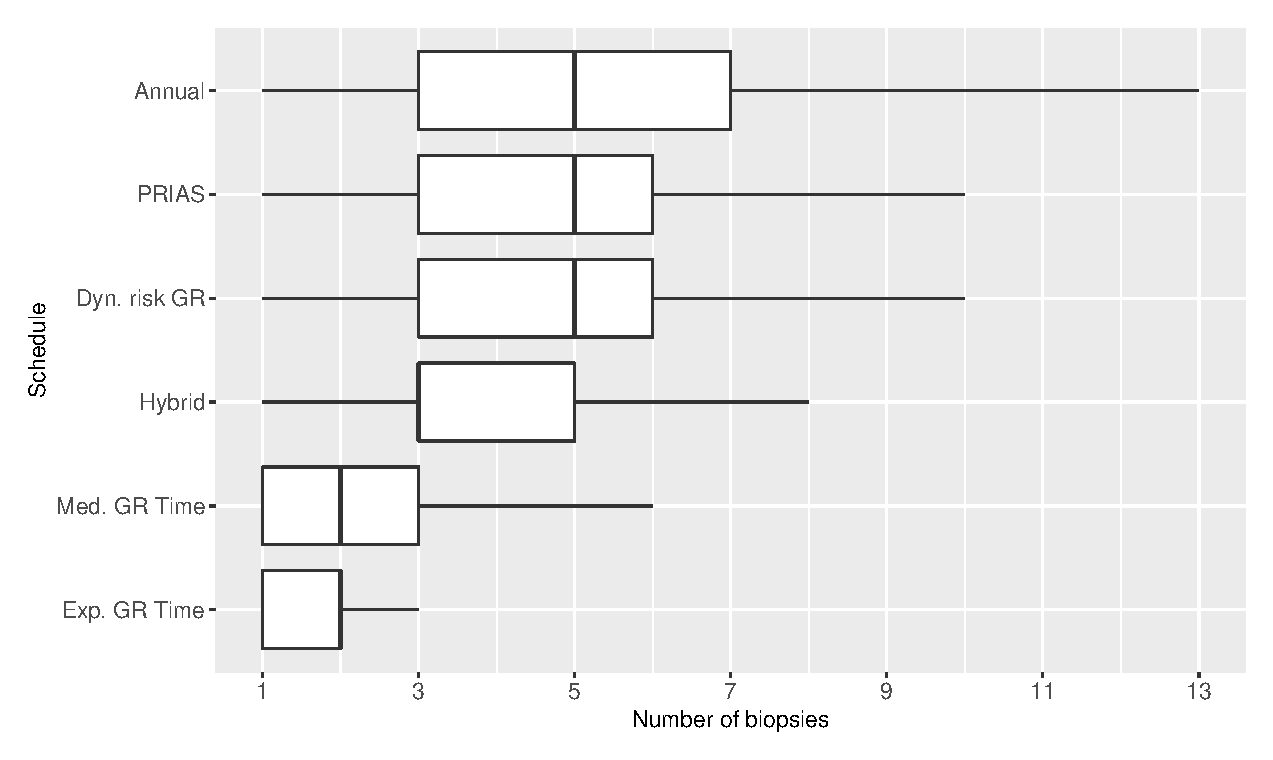
\includegraphics[width=\columnwidth]{images/sim_study/nbBoxPlot_all.eps}}
\caption{Boxplot showing variation in number of biopsies conducted by various schedules, obtained from the simulation study with 500 simulated datasets.}
\label{fig : nbBoxPlot_all}
\end{figure}

\begin{figure}[!htb]
\centerline{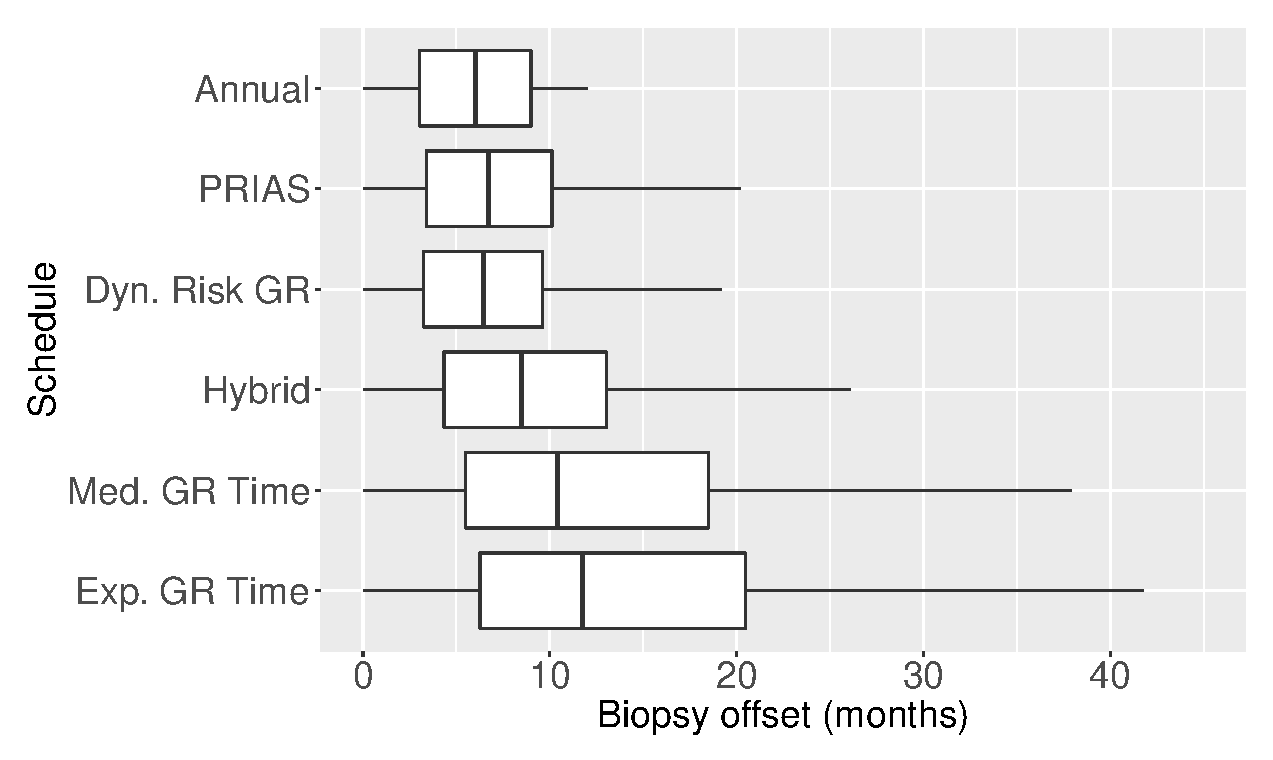
\includegraphics[width=\columnwidth]{images/sim_study/offsetBoxPlot_all.eps}}
\caption{Boxplot showing variation in biopsy offset (months) for various schedules, obtained from the simulation study with 500 simulated datasets.}
\label{fig : offsetBoxPlot_all}
\end{figure}

The choice of a suitable schedule using (\ref{eq : loss_func_sim_study_generic}) depends on the chosen measure for evaluation of schedules. In this regard, the schedules we compared either have high $\mbox{SD}(O^S_j)$ and low $\mbox{SD}(N^S_j)$, or vice versa (Table \ref{table : sim_study_pooled_estimates}). Thus, applying a cutoff on $E(O^S_j)$ when $\mbox{SD}(O^S_j)$ is high may not be as fruitful (same for $N^S_j$) as applying a cutoff on $\mbox{SD}(O^S_j)$ or quantile(s) of $O^S_j$. For example, the schedule based on the dynamic risk of GR is suitable if on average the least number of biopsies are to be conducted to detect GR, while simultaneously making sure that at least 90\% of the patients have an average offset less than one year.


\textbf{}

\clearpage
\printbibliography

\appendix

% !TEX root =  ../main.tex 

\section{Appendix}

\subsection{Personalized schedules for repeat biopsies}
In this section we present the derivations for Equation \ref{eq : expected_time_survprob} and Equation \ref{eq : var_time_survprob}. To this end, we first expand the formula for dynamic survival probability presented in Equation \ref{eq : dynamic_surv_prob}.
\begin{equation}
\label{eq : dyn_surv_prob_expanded}
\begin{split}
\pi_j(u \mid t, s) &= \mbox{Pr}\big\{T^*_j \geq u \mid  T^*_j >t, \mathcal{Y}_j(s\big\}, D_n)\\
&= \int \int \mbox{Pr}\big\{T^*_j \geq u \mid  T^*_j >t, \boldsymbol{b}_j,\boldsymbol{\theta}\big\} p\big(\boldsymbol{b}_j \mid T^*_j>t, \mathcal{Y}_j(s), \boldsymbol{\theta}\big)p\big(\boldsymbol{\theta} \mid \mathcal{D}_n\big) \diff \boldsymbol{b}_j \diff \boldsymbol{\theta}\\
&= \int \int \frac{\exp\big\{-H_j(u | \boldsymbol{b}_j, \boldsymbol{\theta})\big\}}{\exp\big\{-H_j(t | \boldsymbol{b}_j, \boldsymbol{\theta})\big\}} p\big(\boldsymbol{b}_j \mid T^*_j>t, \mathcal{Y}_j(s), \boldsymbol{\theta}\big)p\big(\boldsymbol{\theta} \mid \mathcal{D}_n\big) \diff \boldsymbol{b}_j \diff \boldsymbol{\theta}
\end{split}
\end{equation}
where $H_j(u | \boldsymbol{b}_j, \boldsymbol{\theta}) = \int_0^u h_i(s \mid \boldsymbol{b}_j, \boldsymbol{\theta}\big)\diff s$ is the cumulative hazard up to time point $u$.

\subsubsection{Derivation of Equation \ref{eq : expected_time_survprob}}
\label{subsubsec : deriv_eq_7}
\begin{equation*}
\begin{split}
E_g[T^*_j] &= \int_t^{\infty} T^*_j g(T^*_j)\diff T^*_j\\
\text{Using integration by parts, wherein} & \frac{\diff \big\{-\pi_j(T^*_j \mid t, s)\big\}}{\diff T^*_j} = g(T^*_j)\\
&= \Big[-T^*_j\pi_j(T^*_j \mid t, s)\Big]_t^\infty + \int_t^{\infty} \pi_j(T^*_j \mid t, s) \frac{\diff (T^*_j)}{\diff T^*_j} \diff T^*_j\\
&= t \pi_j(t \mid t, s) - \lim_{T^*_j\to \infty}T^*_j \pi_j(T^*_j \mid t, s) + \int_t^{\infty} \pi_j(T^*_j \mid t, s) \diff T^*_j\\
\end{split}
\end{equation*}
where $\pi_j(t \mid t, s) = \mbox{Pr}\big\{T^*_j \geq t \mid  T^*_j >t, \mathcal{Y}_j(s), D_n\big\} = 1$. As for $\lim_{T^*_j\to \infty}T^*_j \pi_j(T^*_j \mid t, s)$, the limit can be interchanged with the integral in Equation \ref{eq : dyn_surv_prob_expanded}, because as $T^*_j\to \infty$ the integrand in the equation converges uniformly on the domain of $(\boldsymbol{b}_j, \boldsymbol{\theta}\big)$. Thus,
\begin{equation*}
\begin{split}
\lim_{T^*_j\to \infty}T^*_j \pi_j(T^*_j \mid t, s) &=  \int \int \lim_{T^*_j\to \infty} \frac{T^*_j}{\exp\big\{H_j(T^*_j | \boldsymbol{b}_j, \boldsymbol{\theta})\big\}} \frac{p\big(\boldsymbol{b}_j \mid T^*_j>t, \mathcal{Y}_j(s), \boldsymbol{\theta}\big)p\big(\boldsymbol{\theta} \mid \mathcal{D}_n\big)}{\exp\big\{-H_j(t | \boldsymbol{b}_j, \boldsymbol{\theta})\big\}}  \diff \boldsymbol{b}_j \diff \boldsymbol{\theta}\\
\text{Using L'Hospital's rule}\\
\lim_{T^*_j\to \infty}T^*_j \pi_j(T^*_j \mid t, s) &=  \int \int \frac{1}{\lim_{T^*_j\to \infty} \exp\{H_j(T^*_j | \boldsymbol{b}_j, \boldsymbol{\theta}\big)\}H'_j(T^*_j | \boldsymbol{b}_j, \boldsymbol{\theta}\big)} \frac{p\big(\boldsymbol{b}_j \mid T^*_j>t, \mathcal{Y}_j(s), \boldsymbol{\theta}\big)p\big(\boldsymbol{\theta} \mid \mathcal{D}_n\big)}{\exp\{-H_j(t | \boldsymbol{b}_j, \boldsymbol{\theta}\big)\}} \diff \boldsymbol{b}_j \diff \boldsymbol{\theta}\\
&= \int \int 0 \frac{p\big(\boldsymbol{b}_j \mid T^*_j>t, \mathcal{Y}_j(s), \boldsymbol{\theta}\big)p\big(\boldsymbol{\theta} \mid \mathcal{D}_n\big)}{\exp\big\{-H_j(t | \boldsymbol{b}_j, \boldsymbol{\theta})\big\}}  \diff \boldsymbol{b}_j \diff \boldsymbol{\theta}\\
&= 0
\end{split}
\end{equation*}

In light of these results, we obtain:
\begin{equation*}
E_g[T^*_j] = t + \int_t^{\infty} \pi_j(T^*_j \mid t, s) \diff T^*_j\\
\end{equation*}

\subsubsection{Derivation of Equation \ref{eq : var_time_survprob}}
Since $\mbox{var}_g[T^*_j] = E_g[\{T^*_j\}^2] - E_g[T^*_j]^2$, we first show the derivation for $E_g[(T^*_j)^2]$.
\begin{equation*}
\begin{split}
E_g[(T^*_j)^2] &= \int_t^{\infty} (T^*_j)^2 g(T^*_j)\diff T^*_j\\
\text{Using integration by parts, wherein} & \frac{\diff \big\{-\pi_j(T^*_j \mid t, s)\big\}}{\diff T^*_j} = g(T^*_j)\\
E_g\big[\{T^*_j\}^2\big] &= \Big[-\{T^*_j\}^2\pi_j(T^*_j \mid t, s)\Big]_t^\infty + \int_t^{\infty} \pi_j(T^*_j \mid t, s) \frac{\diff (T^*_j)^2}{\diff T^*_j} \diff T^*_j\\
&= t^2 \pi_j(t \mid t, s) - \lim_{T^*_j\to \infty}(T^*_j)^2 \pi_j(T^*_j \mid t, s) + 2 \int_t^{\infty} T^*_j \pi_j(T^*_j \mid t, s) \diff T^*_j\\
&= t^2 + 2 \int_t^{\infty} T^*_j \pi_j(T^*_j \mid t, s) \diff T^*_j
\end{split}
\end{equation*}
Therefore,
\begin{equation*}
\begin{split}
\mbox{var}_g[T^*_j] &= t^2 + 2 \int_t^{\infty} T^*_j \pi_j(T^*_j \mid t, s) \diff T^*_j - \bigg[t^2 +  \Big\{\int_t^\infty \pi_j(T^*_j \mid t, s) \diff T^*_j \Big\}^2 + 2t\int_t^\infty \pi_j(T^*_j \mid t, s) \diff T^*_j \bigg]\\
&=2 \int_t^{\infty} (T^*_j - t) \pi_j(T^*_j \mid t, s) \diff T^*_j -  \Big\{\int_t^\infty \pi_j(T^*_j \mid t, s) \diff T^*_j \Big\}^2
\end{split}
\end{equation*}

\subsection{Simulation study}
This section presents the figures and tables for related to the simulation study results from Section \ref{sec: simulation_study}. More specifically:

\begin{itemize}
  \item Figure \ref{fig : meanNbVsOffset_G1}, Figure \ref{fig : meanNbVsOffset_G2} and Figure \ref{fig : meanNbVsOffset_G3} show plots of average number of biopsies against average offset for each of the 7 scheduling methods present in the simulation study.
  \item Figure \ref{fig : nbBoxPlot_G1} and Figure \ref{fig : offsetBoxPlot_G1} show boxplots of number of biopsies and offset for each of the 6 scheduling methods for the patients in subgroup $G_1$. Similar plots for subgroup $G_2$ and $G_3$ are shown in Figure \ref{fig : nbAndOffsetBoxPlot_G2} and Figure \ref{fig : nbAndOffsetBoxPlot_G3} respectively.
  \item Figure \ref{fig : nbMeanBoxPlot_all} and Figure \ref{fig : offsetMeanBoxPlot_all} show the variation in estimated mean number of biopsies and estimated mean offset computed during the 254 simulations, for patients from all subgroups. The same plots for each of the subgroups are shown in Figure \ref{fig : nbAndOffsetMeanBoxPlot_G1}, Figure \ref{fig : nbAndOffsetMeanBoxPlot_G2} and Figure \ref{fig : nbAndOffsetMeanBoxPlot_G3}.
\end{itemize} 

\begin{figure}[!htb]
    \centering
    \captionsetup{justification=centering}
     \begin{subfigure}[b]{0.45\textwidth}
        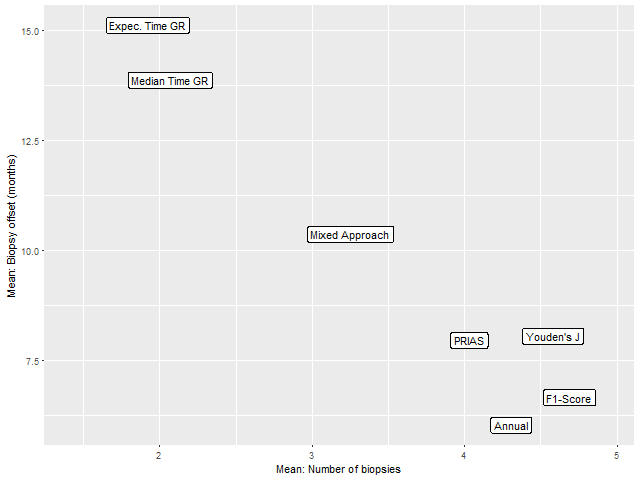
\includegraphics[width=\textwidth]{images/sim_study/meanNbVsOffset_scale_4.png}
		\caption{Plot for subgroup $G_1$}
		\label{fig : meanNbVsOffset_G1}
    \end{subfigure}
    \begin{subfigure}[b]{0.45\textwidth}
		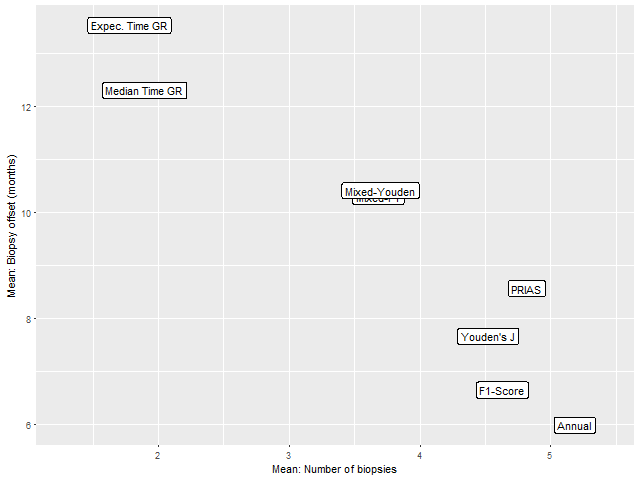
\includegraphics[width=\textwidth]{images/sim_study/meanNbVsOffset_scale_5.png}
		\caption{Plot for subgroup $G_2$}
		\label{fig : meanNbVsOffset_G2}
    \end{subfigure}  
    \begin{subfigure}[b]{0.45\textwidth}
		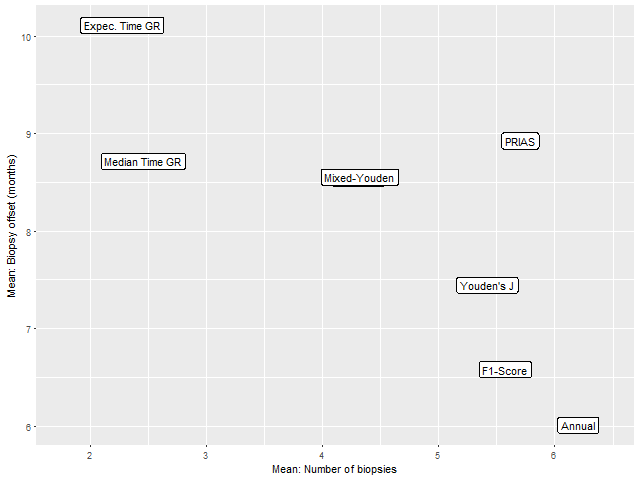
\includegraphics[width=\textwidth]{images/sim_study/meanNbVsOffset_scale_6.png}
		\caption{Plot for subgroup $G_3$}
		\label{fig : meanNbVsOffset_G3}
    \end{subfigure}      
    \caption{Estimated mean number of biopsies and mean offset (months) for the 7 scheduling methods for the 3 sub-groups. Method names are abbreviated for ease of graphing.}
\end{figure}

\begin{figure}[!htb]
    \centering
    \captionsetup{justification=centering}
     \begin{subfigure}[b]{0.45\textwidth}
        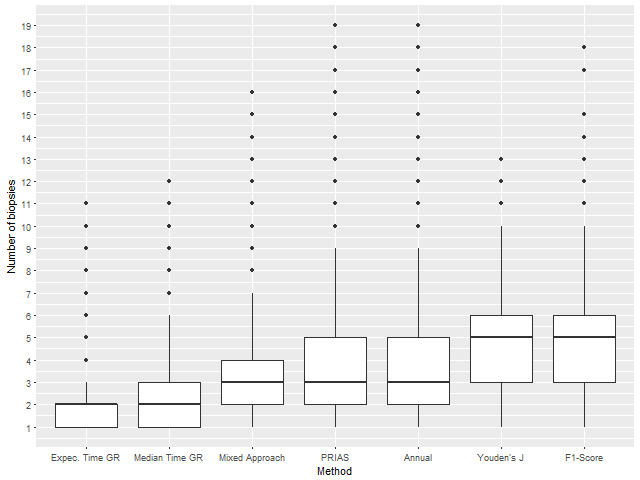
\includegraphics[width=\textwidth]{images/sim_study/nbBoxPlot_scale_4.png}
        \caption{Boxplot for number of biopsies.}
        \label{fig : nbBoxPlot_G1}
    \end{subfigure}
    \begin{subfigure}[b]{0.45\textwidth}
        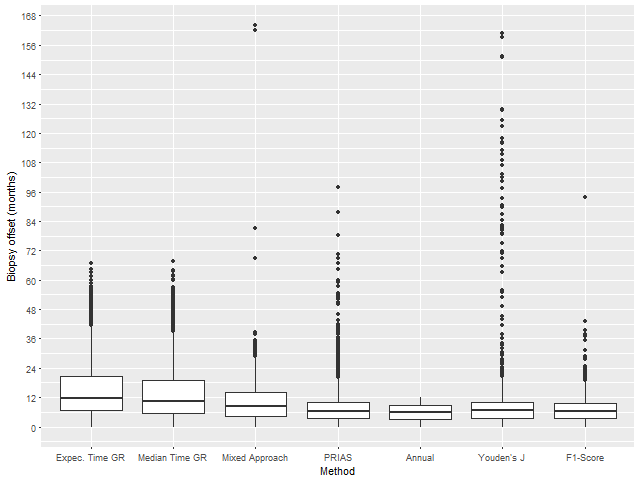
\includegraphics[width=\textwidth]{images/sim_study/offsetBoxPlot_scale_4.png}
        \caption{Boxplot for offset (months)}
        \label{fig : offsetBoxPlot_G1}
    \end{subfigure}      
    \caption{Boxplot for number of biopsies and offset (months), for all patients in subgroup $G_1$ across all simulations. Method names are abbreviated for ease of graphing.}
    \label{fig : nbAndOffsetBoxPlot_G1}
\end{figure}

\begin{figure}[!htb]
    \centering
    \captionsetup{justification=centering}
     \begin{subfigure}[b]{0.45\textwidth}
        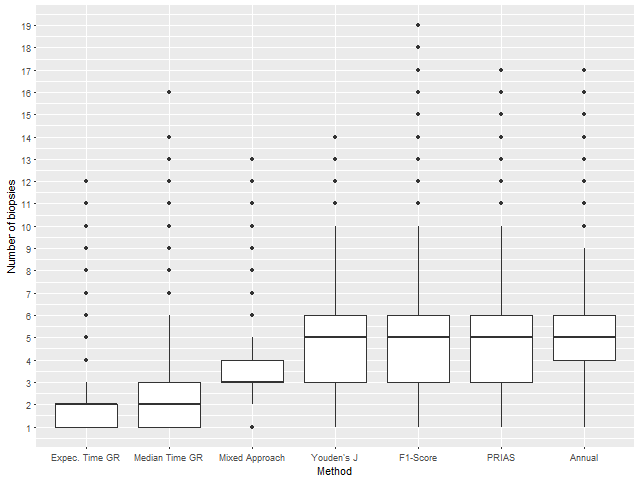
\includegraphics[width=\textwidth]{images/sim_study/nbBoxPlot_scale_5.png}
        \caption{Boxplot for number of biopsies.}
        \label{fig : nbBoxPlot_G2}
    \end{subfigure}
    \begin{subfigure}[b]{0.45\textwidth}
        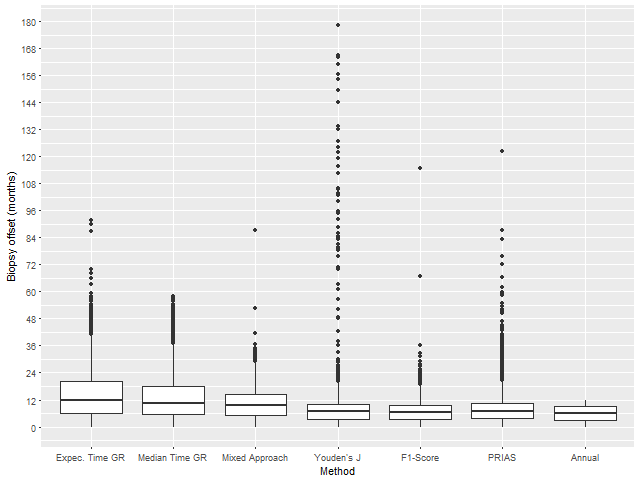
\includegraphics[width=\textwidth]{images/sim_study/offsetBoxPlot_scale_5.png}
        \caption{Boxplot for offset (months)}
        \label{fig : offsetBoxPlot_G2}
    \end{subfigure}      
    \caption{Boxplot for number of biopsies and offset (months), for all patients in subgroup $G_2$ across all simulations. Method names are abbreviated for ease of graphing.}
     \label{fig : nbAndOffsetBoxPlot_G2}
\end{figure}

\begin{figure}[!htb]
    \centering
    \captionsetup{justification=centering}
     \begin{subfigure}[b]{0.45\textwidth}
        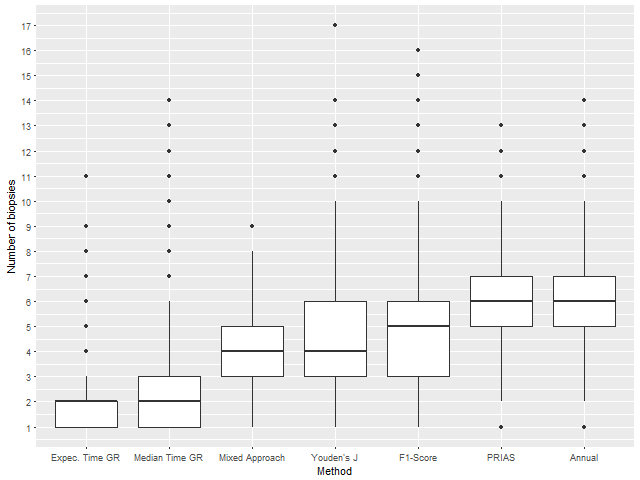
\includegraphics[width=\textwidth]{images/sim_study/nbBoxPlot_scale_6.png}
        \caption{Boxplot for number of biopsies.}
        \label{fig : nbBoxPlot_G3}
    \end{subfigure}
    \begin{subfigure}[b]{0.45\textwidth}
        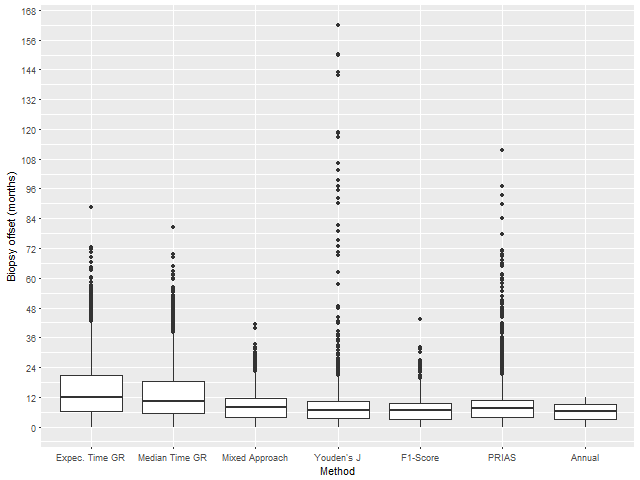
\includegraphics[width=\textwidth]{images/sim_study/offsetBoxPlot_scale_6.png}
        \caption{Boxplot for offset (months)}
        \label{fig : offsetBoxPlot_G3}
    \end{subfigure}      
    \caption{Boxplot for number of biopsies and offset (months), for all patients in subgroup $G_3$ across all simulations. Method names are abbreviated for ease of graphing.}
     \label{fig : nbAndOffsetBoxPlot_G3}
\end{figure}

\begin{figure}[!htb]
    \centering
    \captionsetup{justification=centering}
     \begin{subfigure}[b]{0.45\textwidth}
        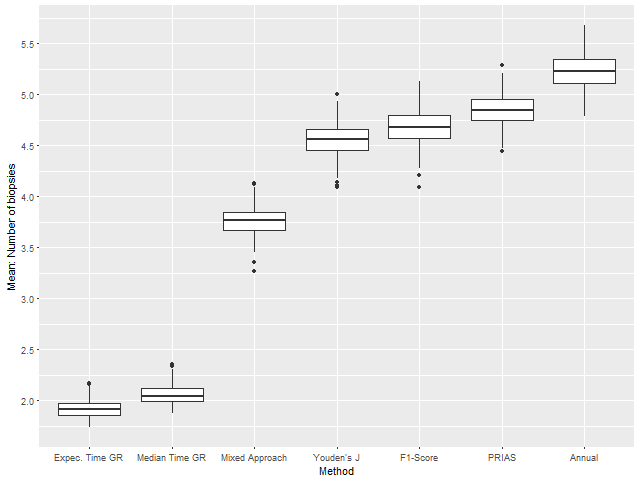
\includegraphics[width=\textwidth]{images/sim_study/nbMeanBoxPlot_all.png}
        \caption{Boxplot for mean number of biopsies.}
        \label{fig : nbMeanBoxPlot_all}
    \end{subfigure}
    \begin{subfigure}[b]{0.45\textwidth}
        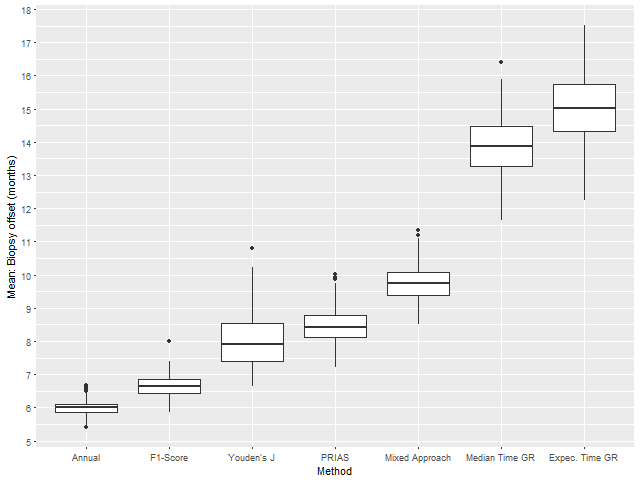
\includegraphics[width=\textwidth]{images/sim_study/offsetMeanBoxPlot_all.png}
        \caption{Boxplot for mean offset (months)}
        \label{fig : offsetMeanBoxPlot_all}
    \end{subfigure}      
    \caption{Boxplot showing variation in mean number of biopsies and mean offset (months) for all of the patients across the 254 simulations.}
\end{figure}

\begin{figure}[!htb]
    \centering
    \captionsetup{justification=centering}
     \begin{subfigure}[b]{0.45\textwidth}
        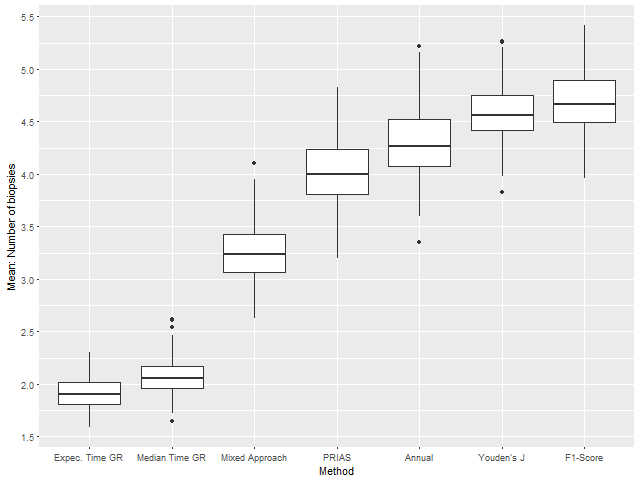
\includegraphics[width=\textwidth]{images/sim_study/nbMeanBoxPlot_scale_4.png}
        \caption{Boxplot for mean number of biopsies.}
        \label{fig : nbMeanBoxPlot_G1}
    \end{subfigure}
    \begin{subfigure}[b]{0.45\textwidth}
        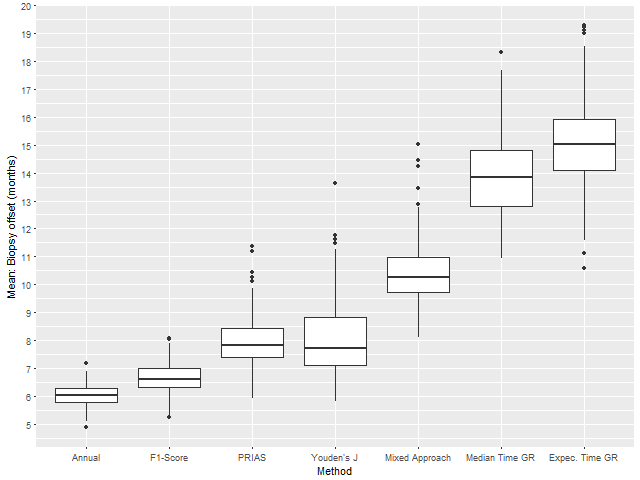
\includegraphics[width=\textwidth]{images/sim_study/offsetMeanBoxPlot_scale_4.png}
        \caption{Boxplot for mean offset (months)}
        \label{fig : offsetMeanBoxPlot_G1}
    \end{subfigure}      
    \caption{Boxplot showing variation in mean number of biopsies and mean offset (months) for patients in subgroup $G_1$ across the 254 simulations.}
    \label{fig : nbAndOffsetMeanBoxPlot_G1}
\end{figure}

\begin{figure}[!htb]
    \centering
    \captionsetup{justification=centering}
     \begin{subfigure}[b]{0.45\textwidth}
        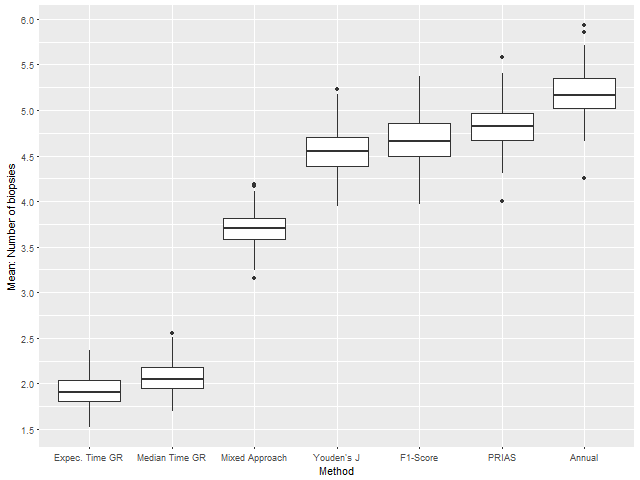
\includegraphics[width=\textwidth]{images/sim_study/nbMeanBoxPlot_scale_5.png}
        \caption{Boxplot for mean number of biopsies.}
        \label{fig : nbMeanBoxPlot_G2}
    \end{subfigure}
    \begin{subfigure}[b]{0.45\textwidth}
        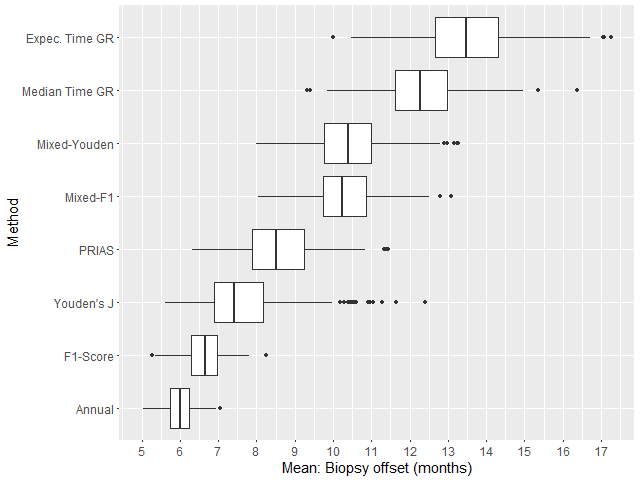
\includegraphics[width=\textwidth]{images/sim_study/offsetMeanBoxPlot_scale_5.png}
        \caption{Boxplot for mean offset (months)}
        \label{fig : offsetMeanBoxPlot_G2}
    \end{subfigure}      
    \caption{Boxplot showing variation in mean number of biopsies and mean offset (months) for patients in subgroup $G_2$ across the 254 simulations.}
    \label{fig : nbAndOffsetMeanBoxPlot_G2}
\end{figure}

\begin{figure}[!htb]
    \centering
    \captionsetup{justification=centering}
     \begin{subfigure}[b]{0.45\textwidth}
        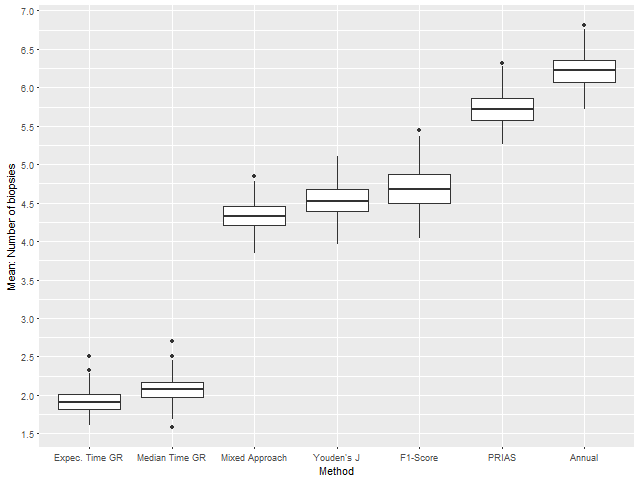
\includegraphics[width=\textwidth]{images/sim_study/nbMeanBoxPlot_scale_6.png}
        \caption{Boxplot for mean number of biopsies.}
        \label{fig : nbMeanBoxPlot_G3}
    \end{subfigure}
    \begin{subfigure}[b]{0.45\textwidth}
        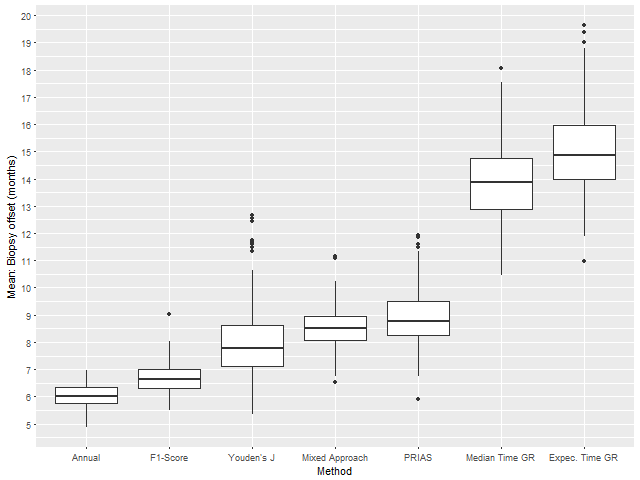
\includegraphics[width=\textwidth]{images/sim_study/offsetMeanBoxPlot_scale_6.png}
        \caption{Boxplot for mean offset (months)}
        \label{fig : offsetMeanBoxPlot_G3}
    \end{subfigure}      
    \caption{Boxplot showing variation in mean number of biopsies and mean offset (months) for patients in subgroup $G_3$ across the 254 simulations.}
    \label{fig : nbAndOffsetMeanBoxPlot_G3}
\end{figure}

\end{document}